
\chapter{简谐振动\label{chap:=007B80=008C10=00632F=0052A8}}

\section{导论\label{sec:8.1_=005BFC=008BBA}}

在对原子核性质进行微观描述时，到目前为止我们仅仅使用了静态的独立粒子模型。我们已经看到，通过合理地定义粒子或准粒子，并采用有效相互作用，我们能够在此类图像下解释许多原子核基态的基本性质。原子核激发能谱对于理解核结构同样极为重要。如果我们在核壳模型内，或在更为精细的独立粒子模型（例如
Hartree-Fock 或 Hartree-Fock-Bogoliubov）内对这些能谱进行分析，便会发现一系列激发态能够非常令人满意地用诸如粒子-空穴（ph）激发或双准粒子激发来解释。然而，也存在大量激发态，其特征根本无法在壳模型激发的框架内予以重现——尽管通过引入涉及对称性破缺的精巧方法，我们已经能够将核子间的重要关联考虑在内。

例如，若我们将讨论局限于球对称双幻核，如 $^{16}\mathrm{O}$、$^{40}\mathrm{Ca}$ 或 $^{208}\mathrm{Pb}$，则根据核壳模型的简谐振子近似，最低的激发能级应当位于约
$1\hbar\omega_{0}$ 处。对于 $^{16}\mathrm{O}$，实验测得的 $1p$ 壳与 $2s\text{-}1d$
壳之间的壳间距大约为 $11.5\,\text{MeV}$。然而，在 $^{16}\mathrm{O}$ 的能谱中，除其他态之外，我们在
$6.14\,\text{MeV}$ 处观察到一个 $(J^{\pi}=3^{-},\,T=0)$ 态；而在约 $22\,\text{MeV}$
处，观察到一个宽约 $5\,\text{MeV}$ 的共振峰，通常称为巨偶极共振（见\ref{fig:8_1}），其量子数为 $J^{\pi}=1^{-},\,T=1$。

\begin{figure}[H]
\begin{centering}
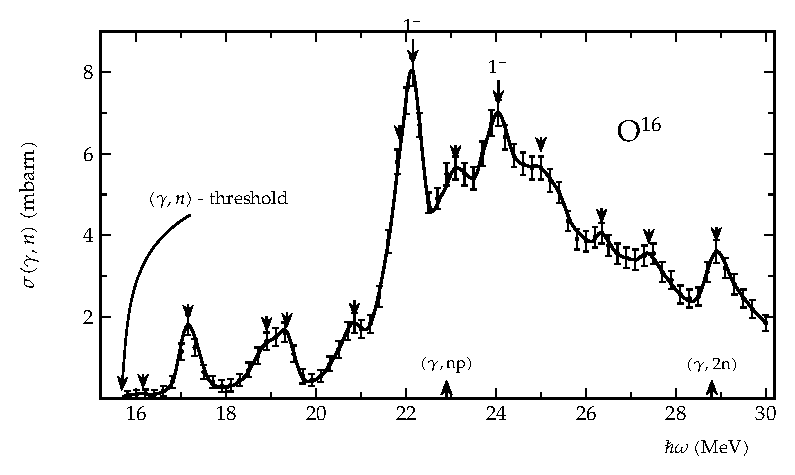
\includegraphics[width=0.8\textwidth]{pictures/8_1}
\par\end{centering}
\caption{\label{fig:8_1}$(\gamma,n)$ 反应截面随 $\gamma$ 能量的变化（引自 \cite{BCH64}）。}
\end{figure}

可以证明（见第 8.3.3 节），该共振主要涉及 $1\hbar\omega$ 激发。因此，纯壳模型同样无法解释巨偶极共振如此之高的能量。

事实表明，只有假定核内大量核子发生了相干协同参与，才能对这些激发做出解释。我们目前对“相干”的理解，还只能借助原子核的经典液滴方法（第
1 章）来表述：人们认为许多核子以类似于核液滴形状振动的方式共同参与运动。在下文中，我们将了解量子力学意义上的相干究竟意味着什么。此外，这类集体激发通常满足以下判据：
\begin{enumerate}
\item 它们的电磁跃迁几率具有集体增强强度，比单粒子跃迁大一到两个数量级（参见第 2.7.2 节）。
\item 它们在元素周期表不同区域各原子核的能谱中展现出极强的规律性。例如，巨偶极共振在整个周期表中均已被观测到，其激发能随质量数缓慢变化［$\propto80A^{-1/3\div-1/6}$，见式
(1.44)］。
\end{enumerate}
球形核以及变形核的能谱中都包含大量满足这些判据的态。我们将把讨论局限于普遍方法上，这些方法在剩余相互作用［式 (2.35)］

\begin{equation}
V_{R}=\frac{1}{4}\sum_{kk',ll'}\bar{v}_{kk'll'}a^{\dagger}_{k}a^{\dagger}_{k'}a_{l'}a_{l}-V_{\text{HF}}\label{eq:tda_residual_interaction}
\end{equation}

的框架下，能够同时解释高激发（通常为共振）以及低激发（通常为束缚态）的集体振动。正如式 (\ref{eq:tda_residual_interaction})
所示，在下文中我们将主要采用 Hartree-Fock 单粒子图像，因为这能使讨论更为简捷。然而必须强调的是，在以下各节中介绍的所有方法，只要采用
HFB 准粒子（参见第 7 章）替代粒子，都可以直接进行推广。在某些特定情况下，我们也会对此做明确展示。

在第 8.2 节中，我们基于无关联的 HF 基态研究 ph 对之间的相互作用（Tamm-Dancoff 近似，TDA）。在第 8.3
节中，介绍不同类型的集体激发。基态关联将在第 8.4 节中于随机相位近似（RPA）框架下加以考虑，并证明 TDA 方法固有的若干困难可以通过这种途径得以解决。在第
8.5 节中，我们将展示如何利用线性响应理论的形式体系推导出相同的方程，以及在处理密度依赖相互作用时会呈现哪些特征。在第 8.6 节中，给出该理论的一些数值应用。求和规则是提取此类共振普适性质、并阐明
RPA-Hamiltonian 量的量子力学本征态与表面振动经典图像之间联系的有力手段，它们将在第 8.7 节中展开讨论。最后，第
8.8 节与第 8.9 节专门讨论 RPA 的特殊推广，如粒子-粒子 RPA 以及准粒子 RPA。

\section{Tamm-Dancoff 方法\label{sec:8.2_Tamm-Dancoff=0065B9=006CD5}\label{sec:8.2_Tamm-Dancoff=008FD1=004F3C}}

\subsection{Tamm-Dancoff 久期方程\label{subsec:8.2.1_Tamm-Dancoff=004E45=00671F=0065B9=007A0B}}

若我们将壳模型势用 $A$ 个核子填充至某个费米能级，如\ref{fig:8_2} 所示，那么所有零、单、双、三、四、$\dots$、$N$
粒子壳模型激发就构成了一组完备的正交基，可用于展开基态 $|0\rangle$ 或激发态 $|\nu\rangle$ 的真实多核子波函数。此时，Schrödinger
方程的精确解可以通过在全壳模型空间中对 $H$ 进行对角化来获得，或者等价地，通过对以下展开系数进行变分来求解。［在下文中，我们约定指标
$m,n$（$i,j$）分别限制在费米面以上（以下）。］

\begin{equation}
|0\rangle=C^{0}_{0}|\text{HF}\rangle+\sum_{mi}C^{0}_{mi}a^{\dagger}_{m}a_{i}|\text{HF}\rangle+\frac{1}{4}\sum_{mnij}C^{0}_{mn,ij}a^{\dagger}_{m}a^{\dagger}_{n}a_{j}a_{i}|\text{HF}\rangle+\cdots\label{eq:tda_expansion_ground}
\end{equation}

\begin{equation}
|\nu\rangle=C^{\nu}_{0}|\text{HF}\rangle+\sum_{mi}C^{\nu}_{mi}a^{\dagger}_{m}a_{i}|\text{HF}\rangle+\frac{1}{4}\sum_{mnij}C^{\nu}_{mn,ij}a^{\dagger}_{m}a^{\dagger}_{n}a_{j}a_{i}|\text{HF}\rangle+\cdots\label{eq:tda_expansion_excited}
\end{equation}

在理想情况下，行列式 $|\text{HF}\rangle$ 应当由填充 Hartree-Fock 势的 $N$ 个最低单粒子能级给出。然而，后者通常用唯象单粒子势来近似。算符
$a^{\dagger}_{m}a_{i}$ 因而湮灭一个费米能级 $\epsilon_{F}$ 之下的粒子（产生一个空穴），并在
$\epsilon_{F}$ 之上产生一个粒子。因此，它被称为粒子-空穴产生算符（\ref{fig:8_2}）。

\begin{figure}[H]
\begin{centering}
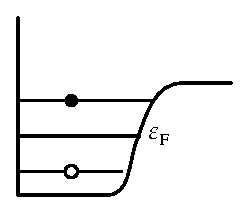
\includegraphics[width=0.5\textwidth]{pictures/8_2}
\par\end{centering}
\caption{\label{fig:8_2}壳模型中的粒子-空穴（ph）激发示意图。}
\end{figure}

在全壳模型空间中精确对角化 $H$ 是一项无法完成的任务。然而，让我们假设在式 (\ref{eq:tda_expansion_excited})
的激发态 $|\nu\rangle$ 展开中，仅保留至 1 粒子-1 空穴（1p-1h）激发是合理的。稍后我们将看到，对于某些类型的状态，这确实是一个极佳的近似。先验地看，也有充分理由说明为何如此：$1\hbar\omega$
粒子-空穴激发子集是能量最低的壳模型组态，因此对于负宇称的低激发态应当极为重要。由电磁场 $F=\sum_{pp'}F_{pp'}a^{\dagger}_{p}a_{p'}$
激发的态的跃迁几率正比于 $|\langle0|F|\nu\rangle|^{2}$，因此这些态被认为具有主导的粒子-空穴贡献。由此我们有理由期望，若在展开式
(\ref{eq:tda_expansion_ground}) 和 (\ref{eq:tda_expansion_excited})
中仅保留以下项：

\begin{equation}
|0\rangle=C^{0}_{0}|\text{HF}\rangle+\sum_{mi}C^{0}_{mi}a^{\dagger}_{m}a_{i}|\text{HF}\rangle\label{eq:tda_ansatz_ground}
\end{equation}

则至少对某一类状态能获得相当不错的近似。由于 $\langle\text{HF}|Ha^{\dagger}_{m}a_{i}|\text{HF}\rangle=0$［式
(5.35)］，我们看到拟设 (\ref{eq:tda_ansatz_ground}) 意味着基态保持为一个行列式，而对于激发态，只需保留

\begin{equation}
|\nu\rangle=\sum_{mi}C^{\nu}_{mi}a^{\dagger}_{m}a_{i}|\text{HF}\rangle\label{eq:tda_ansatz_excited}
\end{equation}

就足够了。这种做法的主要缺点在于：仅在激发态中考虑了关联，而基态保持未关联。稍后我们将看到如何在基态中也建立起关联。

由于 Hamilton 算符与总角动量算符 $\boldsymbol{J}$ 对易，且在很多情况下也与总同位旋算符 $\boldsymbol{T}$
对易，我们理应采用 Clebsch-Gordan 耦合形式的拟设 (\ref{eq:tda_ansatz_excited})［见式
(2.46)］。为了不破坏公式的简明性，除非绝对必要，下文中我们将略去耦合角动量指标。

将式 (\ref{eq:tda_ansatz_excited}) 作为变分拟设，结合

\begin{equation}
\delta\frac{\langle\nu|H|\nu\rangle}{\langle\nu|\nu\rangle}=0\label{eq:tda_variational_principle}
\end{equation}

我们如通常那样得到用于确定本征值和展开系数的久期方程：

\begin{equation}
\sum_{nj}\langle\text{HF}|a^{\dagger}_{i}a_{m}Ha^{\dagger}_{n}a_{j}|\text{HF}\rangle C^{\nu}_{nj}=E_{\nu}C^{\nu}_{mi}\label{eq:tda_secular_matrix}
\end{equation}

利用式 (5.35)，我们可以将式 (\ref{eq:tda_secular_matrix}) 改写为更为便利的形式：

\begin{equation}
\langle\text{HF}|a^{\dagger}_{i}a_{m}[H,a^{\dagger}_{n}a_{j}]|\text{HF}\rangle=(E_{\nu}-E_{\text{HF}})C^{\nu}_{mi}\label{eq:tda_secular_double_commutator}
\end{equation}

式 (\ref{eq:tda_secular_double_commutator}) 中的对易子可利用式 (5.25) 和 (5.26)
容易地求出：

\begin{align}
[H,a^{\dagger}_{n}a_{j}] & =(\epsilon_{n}-\epsilon_{j})a^{\dagger}_{n}a_{j}+\frac{1}{2}\sum_{kl}\left(\bar{v}_{knlj}a^{\dagger}_{n}a^{\dagger}_{k}a_{l}-\bar{v}_{kllj}a^{\dagger}_{k}a^{\dagger}_{l}a_{j}\right)\nonumber \\
 & \quad+\frac{1}{4}\sum_{klm'n'}\bar{v}_{klm'n'}[a^{\dagger}_{k}a^{\dagger}_{l}a_{n'}a_{m'},a^{\dagger}_{n}a_{j}]\label{eq:tda_commutator_h_ph}
\end{align}

利用 Hartree-Fock 单粒子能 $\epsilon$ 的定义式 (5.37) 以及计算场算符基态期望值的规则（附录 C），我们最终得到所谓的
Tamm-Dancoff 方程：

\begin{equation}
(\epsilon_{m}-\epsilon_{i})C^{\nu}_{mi}+\sum_{nj}\bar{v}_{mjin}C^{\nu}_{nj}=E^{\text{TDA}}C^{\nu}_{mi}\label{eq:tda_secular_equation}
\end{equation}

［通过适当选择能量零点，已令 $E_{\text{HF}}=0$，而 $E^{\text{TDA}}$ 是 Tamm-Dancoff
近似（TDA）下 $|\nu\rangle$ 的激发能］。

用图形来表示相互作用的矩阵元通常非常有用：

\begin{equation}
v_{mjin}=\int\mathrm{d}\xi_{1}\mathrm{d}\xi_{2}\phi^{*}_{m}(\xi_{1})\phi^{*}_{j}(\xi_{2})v(\xi_{1},\xi_{2})\phi_{i}(\xi_{1})\phi_{n}(\xi_{2})\label{eq:tda_interaction_integral}
\end{equation}

变量 $\xi$ 象征性地代表全部坐标，且积分包含了对自旋和同位旋的求和。费曼图的绘制规则在许多专著中均有阐述［AGD 63, Ma
67b］；由于我们并不打算将图解法作为一门独立工具来介绍，而仅仅是用作已解析推导内容的直观图示，在此我们不作过多细节铺陈，仅给出绘制约定。波浪线代表
$v$，带箭头的实线代表单粒子波函数（箭头向上代表粒子；箭头向下代表空穴），根据它们的坐标连接到波浪线的相互作用点 1 和 2 上。此外，我们通常约定：在公式
(\ref{eq:tda_interaction_integral}) 中位于相互作用 $v$ 右侧的线指向相互作用点，而左侧的线则背离相互作用点。基于这些约定，$v_{mjin}$
可以用图形展示，如\ref{fig:8_3} 所示。

\begin{figure}[H]
\begin{centering}
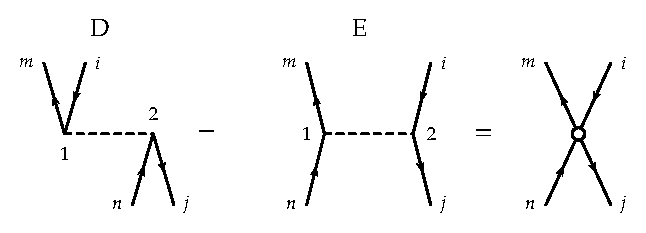
\includegraphics[width=0.75\textwidth]{pictures/8_3}
\par\end{centering}
\caption{\label{fig:8_3}矩阵元 $v_{mjin}$ 与 $v_{mjni}$ 的图形表示。}
\end{figure}

若我们设想垂直于波浪线存在一条时间轴，则在直接项 D 中，一个粒子-空穴对 $nj$ 被湮灭，同时产生了另一个对 $mi$；而在交换项
E 中，粒子-空穴对 $nj$ 散射为一个新的对 $mi$。若将波浪线想象为 $\pi$ 介子，“直接”和“交换”的含义就更加直观了：过程
D 是一个对产生和对湮灭过程（正如电动力学中波浪线代表光子、空穴代表正电子、粒子代表电子那样）；而图 E 则代表在粒子-空穴对之间交换了一个
$\pi$ 介子的过程。通常，直接项与交换项可合并为一个图（Feynman 图），如\ref{fig:8_3} 所示。

\subsection{示意模型\label{subsec:8.2.2_=00793A=00610F=006A21=00578B}\label{subsec:8.2.2_=0096C6=004F53=006027=007684=005224=00636E}}

Tamm-Dancoff 方程的解一般无法在全粒子-空穴空间中求得，因为这是一项极其庞大的数值任务。因此，在大多数情况下仅保留一个“模型空间”，其中包含费米能级
$\epsilon_{F}$ 上下的若干能级。这些计算也常被称为组态混合或壳模型计算。在进入更多细节之前，我们希望在一个极其简明的模型中研究
TDA 方程解的定性特征，在该模型中我们可以得到解析形式的解。

\subsubsection{采用可分离相互作用求解 TDA 方程}

若假定剩余相互作用的矩阵元在粒子-空穴指标上是可分离的（参见第 4.4.7 节及 \cite{BB59,BET61}）：

\begin{equation}
\bar{v}_{mjin}=\chi D_{mi}D^{*}_{nj}\label{eq:tda_separable_force}
\end{equation}

则式 (\ref{eq:tda_secular_equation}) 的求解大为简化。进一步假定 $D_{mi}$ 为某一多极算符（例如四极算符）的矩阵元：

\begin{equation}
D_{mi}=\langle m|r^{2}Y_{2\mu}|i\rangle\label{eq:tda_multipole_element}
\end{equation}

多极阶数自然与粒子-空穴对 $(m,i)$ 耦合到的角动量相一致。矩阵元 (\ref{eq:tda_separable_force})
固然未按严格要求进行反对称化。然而事实证明，交换项很小，将其忽略是一个很好的近似［BK 68, Ma 74］。通常，剩余相互作用对
$T=0$ 态是吸引的（它们的能量被向下推移，例如 $^{16}\mathrm{O}$ 中的 $3^{-},\,T=0$ 态），而对
$T=1$ 态则是排斥的［BB 59］。因此，我们必须选取：

\begin{align}
\chi & <0\quad(\text{对 }T=0),\nonumber \\
\chi & >0\quad(\text{对 }T=1).\label{eq:tda_coupling_sign}
\end{align}

有充分理由表明，相互作用拟设 (\ref{eq:tda_separable_force}) 并不像表面看起来那样简陋，但在此我们不打算深入探讨可分离力的深层物理（见第
4.4.7 节）。相反，我们希望将式 (\ref{eq:tda_separable_force}) 视作一种极为便利的简化，使我们能够探究
TDA 解的定性特征。

基于拟设 (\ref{eq:tda_separable_force})，久期方程 (\ref{eq:tda_secular_equation})
具有如下形式：

\begin{equation}
(E^{\text{TDA}}-\epsilon_{m}+\epsilon_{i})C_{mi}=\chi D_{mi}\sum_{nj}D^{*}_{nj}C_{nj}\label{eq:tda_separable_secular}
\end{equation}

态 $|\nu\rangle$ 当然应当归一化，根据式 (\ref{eq:tda_ansatz_excited})，我们有：

\begin{equation}
\sum_{mi}|C_{mi}|^{2}=1\label{eq:tda_normalization}
\end{equation}

由于 $\sum_{nj}D^{*}_{nj}C_{nj}=\text{const.}$，我们可以从式 (\ref{eq:tda_separable_secular})
中解出展开系数 $C_{mi}$：

\begin{equation}
C_{mi}=N\frac{D_{mi}}{E^{\text{TDA}}-\epsilon_{m}+\epsilon_{i}},\quad N=\left[\sum_{mi}\frac{|D_{mi}|^{2}}{(E^{\text{TDA}}-\epsilon_{m}+\epsilon_{i})^{2}}\right]^{-1/2}\label{eq:tda_separable_coefficients}
\end{equation}

将式 (\ref{eq:tda_separable_secular}) 乘以 $D^{*}_{mi}(E^{\text{TDA}}-\epsilon_{m}+\epsilon_{i})^{-1}$
并对 $m,i$ 求和，便得到决定激发能 $E^{\text{TDA}}$ 的本征值方程：

\begin{equation}
\frac{1}{\chi}=\sum_{mi}\frac{|D_{mi}|^{2}}{E^{\text{TDA}}-\epsilon_{m}+\epsilon_{i}}\label{eq:tda_dispersion_relation}
\end{equation}

我们可以通过绘制右端项随 $E^{\text{TDA}}$ 变化的函数曲线，图形化地求解式 (\ref{eq:tda_dispersion_relation})。由此，本征值就是该函数与水平直线
$1/\chi$ 的交点。所有解都被夹在原始壳模型激发能 $\epsilon_{mi}=\epsilon_{m}-\epsilon_{i}$
之间，唯独有一个解被大幅推高（若 $1/\chi>0$）或大幅拉低（若 $1/\chi<0$）。有限粒子-空穴空间的假设似乎介入了这一论证，但我们必须记住，确定宇称的
ph 壳模型激发聚集为相隔约 $2\hbar\omega_{0}$ 的若干能级簇。因此，\ref{fig:8_4} 仅仅展示了其中一个能级簇。

\begin{figure}[H]
\begin{centering}
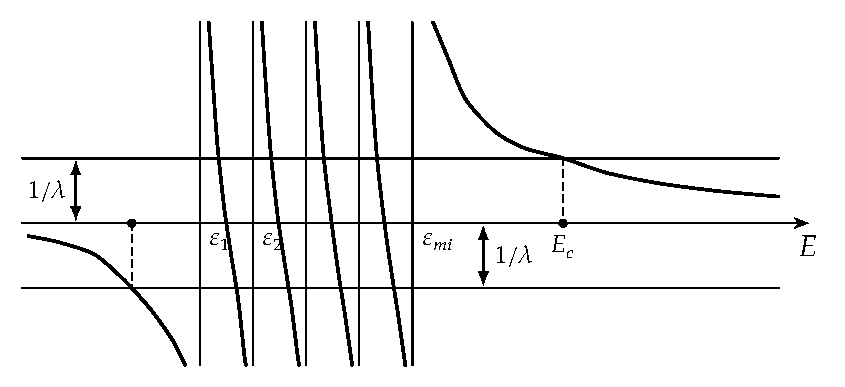
\includegraphics[width=0.75\textwidth]{pictures/8_4}
\par\end{centering}
\caption{\label{fig:8_4}方程 (\ref{eq:tda_dispersion_relation}) 的图解。}
\end{figure}

这一个被显著拉低（$T=0$）或大幅推高（$T=1$）的激发态，是由剩余相互作用的所有矩阵元相干叠加而成的态。这里“相干”的意思是所有矩阵元都以相同的符号做出贡献。这类态的典型例子是在
$^{16}\mathrm{O}$、$^{40}\mathrm{Ca}$ 和 $^{208}\mathrm{Pb}$ 中出现在低激发能处的首个八极态（$T=0$），以及我们稍后将讨论的巨偶极共振（$T=1$）。

\subsubsection{简并情形}

若我们将所有 $\epsilon_{mi}$ 设为相同的值 $\epsilon$，则由式 (\ref{eq:tda_separable_coefficients})
和 (\ref{eq:tda_dispersion_relation}) 容易得出：

\begin{align}
C_{mi} & =\left(\sum_{nj}|D_{nj}|^{2}\right)^{-1/2}D_{mi},\nonumber \\
E^{\text{TDA}} & =\epsilon+\chi\sum_{mi}|D_{mi}|^{2},\label{eq:tda_degenerate_solution}
\end{align}

这意味着集体态被相互作用的所有对角元素之和推高（或拉低）。

这种简并情形可以在例如球形谐振子势（不含自旋-轨道耦合项）中只考虑一个粒子主壳和另一个空穴主壳时实现。在真实原子核中情况不会如此极端，但其本质特征仍很可能得以保持。

对于简并情形，可以通过研究不同激发对总跃迁几率的分配来展现该移动态的集体性。对于集体态，我们有

\begin{equation}
|\text{coll}\rangle=\left(\sum_{mi}|D_{mi}|^{2}\right)^{-1/2}\sum_{mi}D_{mi}a^{\dagger}_{m}a_{i}|\text{HF}\rangle\label{eq:tda_collective_state}
\end{equation}

因此对于跃迁几率，我们得到

\begin{equation}
|\langle\text{coll}|D|0\rangle|^{2}=\left|\left(\sum_{mi}|D_{mi}|^{2}\right)^{-1/2}\sum_{mi}|D_{mi}|^{2}\right|^{2}=\sum_{mi}|D_{mi}|^{2}\label{eq:tda_collective_transition_prob}
\end{equation}

展开系数相干叠加［此处跃迁算符 $D=\sum_{kk'}D_{kk'}a^{\dagger}_{k}a_{k'}$ 应当与可分离相互作用中的算符一致］。

对于所谓的求和规则（参见第 8.7 节），我们得到：

\begin{equation}
\sum_{\nu}|\langle\nu|D|0\rangle|^{2}=\sum_{mi}|\langle mi|D|0\rangle|^{2}=\sum_{mi}|D_{mi}|^{2}\label{eq:tda_sum_rule_exhaustion}
\end{equation}

在此我们将 ph 空间中的完备基 $|\nu\rangle$ 替换为完备基 $|mi\rangle$。对比式 (\ref{eq:tda_collective_transition_prob})
可以看出，总求和规则被集体态完全耗尽。

这意味着在简并情形下，从基态到任何非集体态的跃迁几率均为零。另一方面，到集体态的跃迁几率［式 (\ref{eq:tda_collective_transition_prob})］获得了极大的增强。由此，我们对\ref{fig:8_1}
中所示的强 $1^{-}$ 共振得到了定性解释。

\subsection{粒子-粒子（空穴-空穴）Tamm-Dancoff 方法\label{subsec:8.2.3_=007C92=005B50-=007C92=005B50=00FF08=007A7A=007A74-=007A7A=007A74=00FF09Tamm-Dancoff=0065B9=006CD5}}

正如我们在双幻核情形所看到的，超越 Hartree-Fock 的最简单关联只能通过打破 HF 核心、并将一个核子从费米能级之下提升到其之上来考虑。在远离双幻核时，即通过向下一个开壳填充核子，另一种截然不同的关联就显得至关重要。由于幻核被认为是相当稳定的实体，价核子之间的关联似乎单独决定了关于这些原子核已知的各种实验事实。涵盖从
$^{16}\mathrm{O}$ 到 $^{40}\mathrm{Ca}$ 的 $s\text{-}d$ 壳核也许是此类“开壳”核中研究得最透彻的范例。为了处理这类原子核，人们发展了一整套理论，最广为人知的名称是壳模型组态混合计算。该理论的许多要素可在
de-Shalit 和 Talmi 的专著［ST 63］中找到，而该理论框架下最先进的计算是由 Oak Ridge 组［HMW 71］以及
Whitehead［Wh 72］完成的。在本节中，我们只想讨论这类原子核最简单的情形，即仅偏离闭壳两个粒子，从而填入两个核子或移去两个核子（产生两个空穴）。根据上面的阐述并类比于
ph 情形，我们尝试如下变分拟设（pp-TDA 方法）：

\begin{equation}
|1,A+2\rangle=\sum_{m<n}C^{1}_{mn}a^{\dagger}_{m}a^{\dagger}_{n}|\text{HF}\rangle\label{eq:pptda_ansatz}
\end{equation}

系数 $C_{mn}$ 假定是反对称的，即 $C_{mn}=-C_{nm}$。完全类比于 ph-TDA 情形，我们得到 pp-TDA
久期方程：

\begin{equation}
(E^{\text{TDA}}_{1}-\epsilon_{m}-\epsilon_{n})C^{1}_{mn}=\sum_{m'<n'}\bar{v}_{mnm'n'}C^{1}_{m'n'}\label{eq:pptda_secular_equation}
\end{equation}

这是一个线性 Hermitian 本征值问题。本征矢必须满足归一化与完备性关系（$n<m,\,n'<m'$）：

\begin{equation}
\sum_{m<n}C^{1*}_{mn}C^{1'}_{mn}=\delta_{11'}\label{eq:pptda_orthonormality}
\end{equation}

\begin{equation}
\sum_{1}C^{1}_{mn}C^{1*}_{m'n'}=\delta_{mm'}\delta_{nn'}\label{eq:pptda_closure}
\end{equation}

正如所指出的，原则上求和遍及所有 $>\epsilon_{F}$ 的能级，因此包含了束缚态与连续态。由于这通常会导致矩阵规模超出当今计算机的能力，我们通常在受限子空间中工作，只考虑费米能级之上的一个或两个主壳。为了补偿未包含能级的影响，必须采用适当“重整化”的有效相互作用（参见第
4.3.2 节）。对于 hh-TDA 情形，方程与式 (\ref{eq:pptda_secular_equation}) 完全相同，只需将粒子指标
$(m,n)$ 替换为空穴指标 $(i,j)$，并将单粒子能的符号取反。pp（hh）方程的解可以展现出与 ph 情形相似的特征。例如，我们也可以得到低激发的集体态，通常称为配对振动（参见第
8.3.5 节）。由于定性讨论与 ph 情形非常相似，我们在此不再赘述。（关于铅同位素区域的计算，可参见例如［HK 72, MT 73］及相关文献）。

\section{集体模式的一般考量\label{sec:8.3_=0096C6=004F53=006A21=005F0F=007684=004E00=00822C=008003=0091CF}}

\subsection{量子力学中的振动\label{subsec:8.3.1_=0091CF=005B50=00529B=005B66=004E2D=007684=00632F=0052A8}}

或许现在是暂时中断我们对 TDA 方法多少有些形式化讨论的合适时机，以便更深入地审视集体态的本质。在第 1 章中，我们将这些态描述为液滴的振动。在量子力学语境下，“振动”一词可能会令人困惑，因为我们实际上处理的仅仅是定态。这种定态的密度
$\rho(\boldsymbol{r})$ 是与时间无关的。这里的对应关系大致类似于在量子力学谐振子问题中谈论振荡。为了得到围绕基态密度
$\rho^{(0)}(\boldsymbol{r})$ 振动的含时密度分布 $\rho(\boldsymbol{r},t)$，我们必须研究包含基态
$|0\rangle$ 以及少量激发态 $|\nu\rangle$ 掺杂的波包：

\begin{equation}
|\Psi(t)\rangle=e^{-\mathrm{i}E_{0}t/\hbar}\left(|0\rangle+\sum_{\nu}c_{\nu}e^{-\mathrm{i}\Omega_{\nu}t}|\nu\rangle\right)\label{eq:coll_wavepacket}
\end{equation}

式中 $\hbar\Omega_{\nu}=E_{\nu}-E_{0}$。在系数 $c_{\nu}$ 的一阶近似下，相应的密度为（参见附录
D）：

\begin{align}
\rho(\boldsymbol{r},t) & =\langle\Psi(t)|\sum_{i}\delta(\boldsymbol{r}-\boldsymbol{r}_{i})|\Psi(t)\rangle\nonumber \\
 & =\rho^{(0)}(\boldsymbol{r})+\delta\rho(\boldsymbol{r},t)\label{eq:coll_density_expansion}
\end{align}

其中

\begin{equation}
\delta\rho(\boldsymbol{r},t)=\sum_{\nu}\left(c_{\nu}e^{-\mathrm{i}\Omega_{\nu}t}\rho^{(\nu)}(\boldsymbol{r})+c^{*}_{\nu}e^{\mathrm{i}\Omega_{\nu}t}\rho^{(\nu)*}(\boldsymbol{r})\right)\label{eq:coll_density_variation}
\end{equation}

对该密度进行 Fourier 分析，便可给出不同激发态的贡献：

\begin{equation}
\rho^{(\nu)}(\boldsymbol{r})=\langle0|\sum_{i}\delta(\boldsymbol{r}-\boldsymbol{r}_{i})|\nu\rangle\label{eq:coll_transition_density}
\end{equation}

这些物理量被称为跃迁密度（transition densities）。

一般而言，我们不仅期望如式 (\ref{eq:coll_density_expansion}) 所示在密度的局域部分出现振荡，而且期望在非局域部分也发生振荡，也就是说，我们对跃迁密度矩阵感兴趣。正如附录
D 中所讨论的，在壳模型基下，它具有如下形式：

\begin{equation}
\rho^{(\nu)}_{kk'}=\langle0|a^{\dagger}_{k'}a_{k}|\nu\rangle\label{eq:coll_transition_density_matrix}
\end{equation}

在 TDA 方法中，这些矩阵元由式 (\ref{eq:tda_ansatz_excited}) 中的系数 $C^{\nu}_{mi}$
给出，即在 TDA 中有：

\begin{equation}
\rho^{(\nu)*}_{mi}=C^{\nu}_{mi}\label{eq:coll_tda_density_matrix}
\end{equation}

根据其各种自由度，原子核可以呈现出许多不同类型的运动模式：原子核可以发生形变、平移或压缩；质子与中子的密度可以同相位或反相位振动；在自旋和同位旋自由度上也可以发生振动；我们还有配对模式以及许多其他模式，在下文中我们只能讨论其中若干最基本的模式。

\subsection{集体模式的分类\label{subsec:8.3.2_=0096C6=004F53=006A21=005F0F=007684=005206=007C7B}}

由于本章讨论的是简谐振动，在下文中我们将更详细地探究其定性性质。为了看清其基本结构，我们将讨论局限于球对称闭壳核，最合适的研究范例是
$^{208}\mathrm{Pb}$。然而，这些考量同样适用于元素周期表中的其他区域。事实上，正如我们在导论中所见，许多此类集体激发展现出相当经典的属性，它们平滑地依赖于质量数。

集体粒子-空穴（ph）振动可以通过相应对算符［Mo 76a, b］

\begin{equation}
(a^{\dagger}a)_{J^{\pi}T}\label{eq:coll_pair_operator}
\end{equation}

的性质来表征。Hamiltonian 量具有若干精确对称性，例如转动不变性、宇称守恒以及电荷守恒，对应着量子数 $J$、$\pi$
和 $T_{z}$。此外，对于轻核和重核，我们还拥有（正如第 2.6.3 节中所讨论的）带有量子数 $T$ 的近似同位旋对称性。由于我们从处于基态（$J^{\pi}=0^{+}$）的球形闭壳核出发，激发的角动量与宇称完全由耦合对
$(a^{\dagger}a)_{J^{\pi}}$ 的相应量子数所决定。对于轻核（$N=Z$，基态 $T=0$），同位旋的情况亦是如此。对于重核，基态的同位旋为
$T_{0}=(N-Z)/2$，它必须与 ph 对的同位旋耦合成总同位旋 $T=T_{0}$ 或 $T=T_{0}+1$\footnote{$T=T_{0}-1$ 仅在质子粒子-中子空穴激发中才可能出现，对应于相邻奇奇核中的状态。}。我们通常根据
ph 对 $a^{\dagger}a$ 的同位旋变化 $\Delta T$ 对激发进行分类。因此，我们有 $\Delta T=0$
或 $\Delta T=1$ 激发；并且 $\Delta T=1$ 的激发并不必然意味着 $T=T_{0}+1$。

除了这些给出例如角分布信息的关于对称性的一般考量之外，我们还希望根据 ph 对

\begin{equation}
a^{\dagger}(\boldsymbol{r},s,\tau)a(\boldsymbol{r}',s',\tau')\label{eq:coll_general_ph_density}
\end{equation}

中的不同自由度，对集体运动进行更为精确的分类：

(a) 首先，存在原子核局域密度 $\rho(\boldsymbol{r})$ 在空间中的振动。由于此类振动的角度依赖性已完全由角动量决定，我们只需考虑不同的径向形状。在此语境下最简单的例子是具有清晰表面的球体表面振动，我们在第
1.4 节中对此进行了非常详尽的讨论。由式 (1.7) 可以发现，对于这种具有清晰表面的表面振动，跃迁密度 (\ref{eq:coll_transition_density})
给出为：

\begin{equation}
\rho^{(\nu)}(\boldsymbol{r})=\begin{cases}
\rho_{0}, & r\text{ 介于 }R_{0}\text{ 与 }R(\theta,\phi)\text{ 之间},\\
0, & \text{其他区域},
\end{cases}\label{eq:coll_sharp_surface_transition_density}
\end{equation}

即核内部的密度保持恒定，整个跃迁全部集中在表面区域。我们也可以设想 $\rho^{(\nu)}(\boldsymbol{r})$
具有其他径向依赖形式，其中内部密度也发生改变。这类激发被称为呼吸模（breathing modes）。

(b) 另一种截然不同的运动类型同样仅涉及空间自由度，即跃迁密度矩阵非局域部分 $\rho^{(\nu)}(\boldsymbol{r},\boldsymbol{r}')$
的振动。一个典型的例子是原子核扭曲模（twist mode），其中原子核的局域密度保持不变，仅仅内禀速度分布发生振荡（参见［HE 77］）。

(c) 同位旋是一个额外的自由度。在此我们必须区分同一原子核内的激发（$\Delta T_{z}=0$）与同位旋翻转过程（$\Delta T_{z}=-1$），后者属于电荷为
$Z+1$、中子数为 $N-1$ 的相邻原子核。在第一种情况下，ph 对可以耦合为 $\Delta T=0$ 或 $\Delta T=1$。因此，对于迄今讨论的所有模式我们都有两种选择：质子与中子同相位振动（$\Delta T=0$，同位旋标量模），或质子与中子反相位振动（$\Delta T=1$，同位旋矢量模）。在固定空间点
$\boldsymbol{r}$ 处，我们最终会观察到电荷分布的振荡，这对应于核内的极化波。$\Delta T_{z}=-1$
的振动情形是类似共振（模拟共振），将在第 8.3.4 节中展开讨论。

(d) 最后，我们还拥有自旋自由度。相应的振动产生自旋波。

迄今给出的不同模式的分类，在很大程度上基于坐标空间中的考量，并强调了其经典方面。然而在真实的有限核中，这些模式并未得到完全纯粹的实现。总是或多或少存在非集体态的剧烈掺杂。因此，采用基于最简形式壳模型——简谐振子——的截然不同的分类方法通常极其有用。

\ref{fig:8_5} 示意性地展示了闭壳核（如 $^{208}\mathrm{Pb}$）的壳层结构。我们具有正负宇称交替的壳层，彼此之间相隔约
$1\hbar\omega_{0}$ 的能量距离。对于闭壳核，费米面恰好位于两个壳层之间，因此我们发现负宇称的 $1\hbar\omega_{0}$
激发 ph 对，正宇称的 $2\hbar\omega_{0}$ 激发，负宇称的 $3\hbar\omega_{0}$ 激发等等。对于处于闭壳之间的原子核，我们此外还在壳层内部拥有
$0\hbar\omega_{0}$ 激发。

\begin{figure}[H]
\begin{centering}
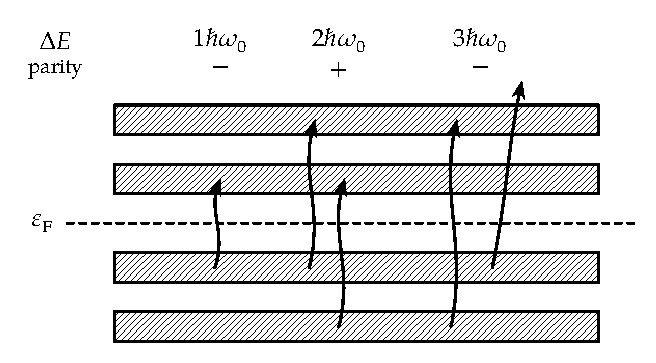
\includegraphics[width=0.75\textwidth]{pictures/8_5}
\par\end{centering}
\caption{\label{fig:8_5}闭壳核中壳层结构与可能出现的 1p-1h 激发示意图。}
\end{figure}

在真实原子核中，简并的振子壳层发生分裂，少数具有“错误”宇称的能级由于自旋-轨道耦合项 $\boldsymbol{l}\cdot\boldsymbol{s}$
的作用向下移入较低的壳层中。这也导致了闭壳核（如 $^{208}\mathrm{Pb}$）中出现正宇称的 $1\hbar\omega_{0}$
激发。但该图像的基本特征在真实情形下依然成立。

虽然在集体激发中存在众多 ph 对的叠加，且由于关联效应产生如第 8.2.2.2 节所讨论的剧烈能量移动，但这种粗粒度结构在很大程度上仍得以保留\footnote{类比于第 8.2.2.2 节，在包含若干简并能级簇的示意模型中同样可以在解析上证明这一点。}。例如对于
$J^{\pi}=3^{-}$，我们发现一个主要由 $1\hbar\omega_{0}$ 激发组成的强集体态，以及另一个主要由
$3\hbar\omega_{0}$ 激发构成的集体态［MNS 76, St 79］。

显而易见，这种壳层结构对低激发集体态的激发能（示意性地显示于图 1.6 中）有着巨大的影响，因为它们紧密依赖于最低 ph 对的粒子-空穴能量。事实上，在这里我们观察到了剧烈的壳效应（见图
1.7）。对于高激发态——巨共振——情况不再如此。两个主壳之间的能量距离在整个周期表上只是平滑地变化［$\hbar\omega_{0}\propto A^{-1/3}$；见式
(2.12)］。因此，我们预期巨共振的共振能量同样表现出平滑的 $A$ 依赖关系。

\subsection{若干集体 ph 振动的讨论\label{subsec:8.3.3_=0082E5=005E72=0096C6=004F53ph=00632F=0052A8=007684=008BA8=008BBA}}

在某种意义上，最平凡的集体运动是由线动量 $\boldsymbol{P}$ 生成的整个原子核的平移运动。由于 $\boldsymbol{P}$
与两体 Hamiltonian 量 $H$ 对易，精确基态 $|0\rangle$ 必定是 $\boldsymbol{P}$
的本征函数。然而，若我们对基态采用破坏了这一对称性的近似态 $|0\rangle_{\text{app}}$，则 $\boldsymbol{P}|0\rangle_{\text{app}}$
就是新的状态。它们看起来类似于集体激发。我们称它们为赝态（spurious states），因为它们并不对应于真实的物理激发。在角动量耦合方案下，它们的量子数为
$J^{\pi}=1^{-},\,T=0$（$\boldsymbol{P}$ 是与同位旋无关的矢量算符）。它们对应于整个原子核的质心平移。由于这种运动不存在恢复力，它们的激发能量理论上应当严格为零：

\begin{equation}
E(1^{-},T=0)-E_{0}=0\label{eq:coll_spurious_energy_zero}
\end{equation}

然而，这取决于具体的理论近似。例如在 TDA 中，$\boldsymbol{P}|\text{HF}\rangle$ 是粒子-空穴态的叠加，通常并不是
TDA 方程 (\ref{eq:tda_secular_equation}) 的本征态。相反，它是所有 TDA 本征态的混合物，这些本征态在
1p-1h 空间中构成完备组。由于其能量仍然接近 $E_{0}$［式 (\ref{eq:coll_spurious_energy_zero})］，它在低激发
TDA 态中占有很大成分。这意味着 TDA 的某些低激发解将严重受到赝态成分的污染。在第 8.4.7 节中我们将看到，RPA 能够优雅地消除这一缺陷。

另一类极为重要的 $1^{-}$ 模式是同位旋矢量偶极振动（$T=1$）。在此模式中，质子与中子相互逆向振动，形成了经典的巨偶极共振（GDR）。在形变核中，我们观察到两种偶极振动，分别平行于对称轴与垂直于对称轴。这种能量的分裂使得人们能够通过实验测定形变参数［Da
58, Ok 58, BBC 71］。

巨偶极共振可以通过例如 $\gamma$ 辐射的光吸收来激发。在附录 B.7 中，我们推导了能量为 $E$ 的光子激发末态 $|\nu\rangle$
的截面：

\begin{equation}
\sigma_{\nu}(E)=\frac{4\pi^{2}e^{2}}{\hbar c}(E_{\nu}-E_{0})|\langle\nu|D|0\rangle|^{2}\delta(E-(E_{\nu}-E_{0}))\label{eq:coll_photo_cross_section_nu}
\end{equation}

式中 $D$ 为沿 $z$ 方向的 E1 辐射偶极算符［式 (B.88)］：

\begin{equation}
D=\frac{NZ}{A}\left(\frac{1}{Z}\sum^{Z}_{p=1}z_{p}-\frac{1}{N}\sum^{N}_{n=1}z_{n}\right)\label{eq:coll_dipole_operator_relative}
\end{equation}

它正比于质子质心与中子质心之间距离的 $z$ 分量。

偶极吸收的总截面 $\sigma_{\text{total}}$ 可通过将式 (\ref{eq:coll_photo_cross_section_nu})
对所有末态 $|\nu\rangle$ 求和并对能量积分得到：

\begin{equation}
\int\sigma_{\gamma}(E)\,\mathrm{d}E=\frac{4\pi^{2}e^{2}}{\hbar c}S_{1}(D)\label{eq:coll_integrated_cross_section}
\end{equation}

它正比于能量加权偶极求和规则（参见第 8.7 节）：

\begin{equation}
S_{1}(D)=\sum_{\nu}(E_{\nu}-E_{0})|\langle\nu|D|0\rangle|^{2}\label{eq:coll_energy_weighted_sum_rule_def}
\end{equation}

且可以写为闭合形式：

\begin{equation}
S_{1}(D)=\frac{1}{2}\langle0|[D,[H,D]]|0\rangle\label{eq:coll_double_commutator_dipole}
\end{equation}

式中 $H$ 为精确两体 Hamiltonian 量，$|0\rangle$ 为精确基态。假定两体相互作用势不具速度依赖性且不包含交换混合（Wigner
力），类比于式 (8.158)，我们很容易求出：

\begin{equation}
\langle0|[D,[H,D]]|0\rangle=\frac{\hbar^{2}}{m}\frac{NZ}{A}\label{eq:coll_tr_sum_rule_eval}
\end{equation}

因此对于偶极求和，我们得到了著名的 Thomas-Reiche-Kuhn（TRK）求和规则：

\begin{equation}
\int\sigma_{\gamma}(E)\,\mathrm{d}E=\frac{2\pi^{2}e^{2}\hbar}{mc}\frac{NZ}{A}\approx0.06\frac{NZ}{A}\,[\text{MeV}\cdot\text{barn}]\label{eq:coll_trk_sum_rule}
\end{equation}

若两体相互作用包含交换混合（参见例如 Brenig［Br 65b］）以及张量力［WKB 73］，该值还会增大 40\%–80\%，从而能够非常准确地重现实验上能量积分总截面的量级。在
$^{16}\mathrm{O}$ 中，偶极求和规则大约只有 3\% 分布在 $20\,\text{MeV}$ 以下的低激发 $1^{-}$
态（它们几乎是纯壳模型 ph 共振）中，而巨共振主峰则集中了约 50\%，清晰地反映了其集体特征。求和规则的其余部分分布在 $30\,\text{MeV}$
以上［ABC 63, FH 62a, b, Ha 65b, BS 64, ADW 78］。对于重核，巨偶极共振甚至能耗尽高达 100\%
的求和规则。实验表明，偶极求和规则 (\ref{eq:coll_trk_sum_rule}) 的绝大部分被巨偶极共振所耗尽，这意味着该共振态与如下态：

\begin{equation}
|D\rangle=D|0\rangle\label{eq:coll_goldhaber_teller_state}
\end{equation}

具有巨大的重叠，该态被称为 Goldhaber-Teller 态［GT 48］（参见第 13.3.3 节）。

态 $|D\rangle$ 的量子数与巨共振 $J^{\pi}=1^{-}$ 相同。在同位旋方面，我们需要区分两种情形：

(a) 对于轻的 $N=Z$ 核，Coulomb 力可以忽略。基态 $|0\rangle$ 的同位旋为 $T=0$。从式 (B.88)
可以看出算符 $D$ 是同位旋空间中的矢量，角动量耦合规则表明 $D|0\rangle$ 具有 $T=1$。

(b) 对于重核，同位旋同样是守恒的。基态具有 $T_{0}=(N-Z)/2$。利用第 2.6.3 节中的类似论证，我们可以证明
$T_{+}|D\rangle=0$，从而确信偶极态 $|D\rangle$ 具有相同的同位旋 $T_{0}$。但这并不意味着原子核的激发能谱中不存在
$T=T_{0}+1$ 的其他 $1^{-}$ 态，只是我们无法通过偶极 $\gamma$ 射线将它们激发出来。

算符 $D$ 的结构表明，巨偶极共振主要由 $1\hbar\omega_{0}$ 激发组成。由于剩余相互作用的排斥性质，它被推移至更高的能量处。

除了这一广为人知的偶极态之外，近年来人们还发现了许多其他更高多极阶数的巨共振。巨四极共振尤其在整个元素周期表上得到了确立，其能量略低于巨偶极共振［PW
71, FT 72, LB 72, HGA 74, Sa 74, KWB 75, YMR 76, Be 76］：

\begin{equation}
E_{2^{+}}\approx60\sim65A^{-1/3}\,[\text{MeV}]\label{eq:coll_gqr_energy}
\end{equation}

这对应于同位旋标量巨四极共振（$T=0$），主要由 $2\hbar\omega_{0}$ 激发构成，由于吸引相互作用而被拉低。能量更高的同位旋矢量四极共振（$T=1$）位于约
$130A^{-1/3}\,\text{MeV}$ 处。此外，巨单极共振（呼吸模，$J^{\pi}=0^{+},\,T=0$）位于约
$80A^{-1/3}\,\text{MeV}$ 处，提供了直接提取核物质不可压缩模量 $K$ 的珍贵实验信息。磁共振（由涉及自旋与轨道角动量的算符激发，$J^{\pi}=1^{+},2^{-},\dots$）以及
Gamow-Teller 激发同样构成了巨共振谱的重要组成部分。在\ref{fig:8_6} 中，我们展示了基于微观 RPA 波函数计算得到的
$^{208}\mathrm{Pb}$ 在巨共振能区的非弹性电子散射谱 $(e,e')$。可以清楚地看到，总散射谱是由多种截然不同的共振结构复杂叠加而成的。

\begin{figure}[H]
\begin{centering}
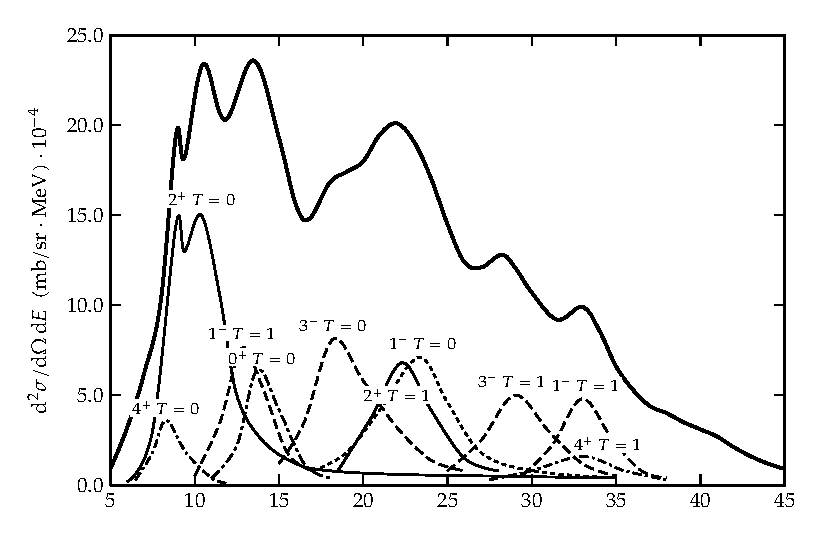
\includegraphics[width=0.8\textwidth]{pictures/8_6}
\par\end{centering}
\caption{\label{fig:8_6}基于微观 RPA 波函数计算得到的 $^{208}\mathrm{Pb}$ 在 $75^{\circ}$
散射角下 $90\,\text{MeV}$ 电子散射 $(e,e')$ 谱。图中的数字标明了相应截面贡献的角动量、宇称与同位旋。}
\end{figure}


\subsection{类似共振\label{subsec:8.3.4_=007C7B=004F3C=005171=00632F}}

重核（$N>Z$）的核反应（例如 $^{208}\mathrm{Pb}(p,n)^{208}\mathrm{Bi}$）表现出强烈的集体共振，由于我们即将阐述的原因，它们被称为类似态（analog
states）\footnote{相关文献可参见例如［AHK 72］。}。

为了解释这些态的结构，我们利用重核波函数在极佳近似下是同位旋算符 $\boldsymbol{T}^{2}$ 本征态的事实（参见第
2.6.3 节）。基态与低激发态具有量子数 $T=T_{z}=(N-Z)/2$。从能量为 $E_{n}$ 的态 $|I,T,T_{z}=T\rangle$
出发，我们可以通过施加同位旋降算符 $T_{-}$ 来定义其类似态：

\begin{equation}
T_{-}|I,T,T_{z}=T\rangle=\sqrt{2T}|I,T,T_{z}=T-1\rangle\label{eq:coll_analog_state_def}
\end{equation}

它属于“子核”（$N-1,Z+1$），且仍然是 $H$ 的本征态，能量为：

\begin{equation}
E_{A}=E_{n}+\Delta_{C}\label{eq:coll_analog_energy}
\end{equation}

为了理解这一点，我们将精确 Hamiltonian 量 $H$ 分解为与 $T_{-}$ 对易的强核力部分 $H_{\text{nucl}}$
以及 Coulomb 相互作用 $V_{c}$：

\begin{equation}
HT_{-}=(H_{\text{nucl}}+V_{c})T_{-}=T_{-}H+[V_{c},T_{-}]\label{eq:coll_ht_minus_commutator}
\end{equation}

对易子 $[V_{c},T_{-}]$ 具有如下形式：

\begin{equation}
[V_{c},T_{-}]=\sum^{A}_{i=1}v_{c}(i)t_{-}(i)\label{eq:coll_vc_tminus_commutator}
\end{equation}

式中平均 Coulomb 势为：

\begin{equation}
v_{c}(i)=\sum_{j\ne i}\frac{e^{2}}{|\boldsymbol{r}_{i}-\boldsymbol{r}_{j}|}\left(\frac{1}{2}-t_{z}(j)\right)\label{eq:coll_average_coulomb_potential}
\end{equation}

假定该单粒子势在核内部具有约 $\Delta_{C}$ 的常数值（参见图 2.7），我们便得到：母核（$N,Z$）的每个本征态
$|n\rangle$ 都在子核（$N-1,Z+1$）中对应着一个类似态 $T_{-}|n\rangle$：

\begin{equation}
HT_{-}|n\rangle=E_{n}T_{-}|n\rangle+[H,T_{-}]|n\rangle\approx(E_{n}+\Delta_{C})T_{-}|n\rangle\label{eq:coll_analog_schrodinger}
\end{equation}

这意味着在子核中存在一系列能级序列，其能级间距与母核本身的低激发能级完全相同，其同位旋为：

\begin{equation}
T=\frac{N-Z}{2}=\frac{(N-Z-2)}{2}+1\label{eq:coll_analog_isospin_plus_one}
\end{equation}

这比子核基态的同位旋大一个单位（\ref{fig:8_7}）。

\begin{figure}[H]
\begin{centering}
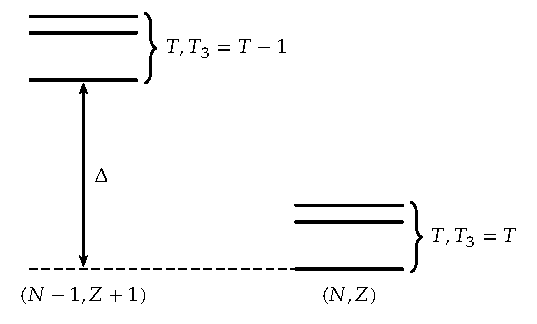
\includegraphics[width=0.5\textwidth]{pictures/8_7}
\par\end{centering}
\caption{\label{fig:8_7}类似态能谱示意图。}
\end{figure}

为了进一步了解类似共振的结构，我们暂时忽略在描述母核（$N,Z$）基态时所使用的剩余相互作用。后者由纯壳模型描述给出，如\ref{fig:8_8}
所示。

\begin{figure}[H]
\begin{centering}
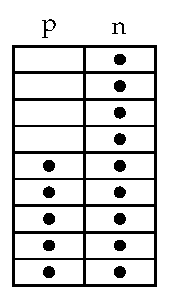
\includegraphics[width=0.25\textwidth]{pictures/8_8}
\par\end{centering}
\caption{\label{fig:8_8}纯壳模型行列式波函数的示意图。}
\end{figure}

我们假设占据相同量子数（除 $t_{z}$ 外）态的质子与中子构成一个惰性核心，并耦合为 $T=0$。在下文中我们将忽略该惰性核心，因此母核的基态由过剩中子描述。利用
$T_{-}=\sum_{i}t_{-}(i)$，我们得到子核的类似态：

\begin{equation}
|I,T,T_{z}=T-1\rangle=\frac{1}{\sqrt{2T}}T_{-}|I,T,T_{z}=T\rangle=\frac{1}{\sqrt{2T}}\sum_{k}a^{\dagger}_{pk}a_{nk}|0\rangle\label{eq:coll_analog_state_ph_expansion}
\end{equation}

式 (\ref{eq:coll_analog_state_ph_expansion}) 中的类似态是某些特定电荷交换粒子-空穴态的相干叠加，这些态是通过将母核基态中的中子逐个替换为处于相应单粒子态的质子而形成的。

当然，还存在与类似态 $|I,T,T_{z}=T-1\rangle$ 正交的其他态 $|A\rangle$，算符 $T_{+}$
将它们完全湮灭，因此它们必须具有同位旋 $T-1$，即子核基态的同位旋。在没有剩余相互作用时，它们与类似态简并并具有相同的自旋与宇称。在实验上，类似态表现为高能量处的极其尖锐的共振峰［AW
61］。它们的宽度之所以如此之小，是因为同位旋选择定则禁止其迅速衰变到构成连续谱背景的其他态中。

\subsection{对振动\label{subsec:8.3.5_=005BF9=00632F=0052A8}}

粒子-粒子相互作用不仅能将核子束缚在一起，还能在核反应中诱发出显著的集体效应。例如在 $^{208}\mathrm{Pb}(p,t)^{206}\mathrm{Pb}$
拾取反应或 $^{208}\mathrm{Pb}(t,p)^{210}\mathrm{Pb}$ 剥离反应截面中［Gl 65］，实验观测到
$^{206}\mathrm{Pb}$ 的 $0^{+}$ 基态的布居几率比 $^{206}\mathrm{Pb}$ 的其他
$0^{+}$ 态大整整一个数量级，这清楚地表明了 $C^{0^{+}}_{ij}$ 振幅的相干贡献以及该状态的强烈集体性。$^{210}\mathrm{Pb}$
的情形与此完全类似。处于 $0^{+}$ 态的两个粒子之间的这种强束缚实体源于相互作用的短程吸引部分，在第 6 章的开头已经对此进行了讨论。两个核子构成了如此稳定的配对实体，以至于它们可以像独立粒子一样（由于其整数自旋，其行为非常类似于玻色子）被成对地加到原子核（如
$^{208}\mathrm{Pb}$）中，或从中移除。因此，其能谱应当近似呈现出简谐振子的阶梯结构，而在铅同位素中实验观测确实如此（\ref{fig:8_9}）［BM
75］。这种谐振谱被称为“配对振动谱”（pairing vibrations）。

\begin{figure}[H]
\begin{centering}
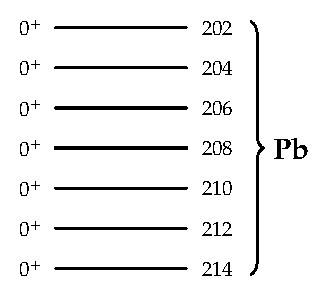
\includegraphics[width=0.4\textwidth]{pictures/8_9}
\par\end{centering}
\caption{\label{fig:8_9}偶数铅同位素基态能量的示意图。}
\end{figure}

我们同样可以在这些核中产生激发的 $0^{+}$ 对振动态。例如，从 $^{208}\mathrm{Pb}$ 中移除一个 $0^{+}$
配对声子使我们到达 $^{206}\mathrm{Pb}$；同时，加上一个从 $^{208}\mathrm{Pb}$ 到 $^{210}\mathrm{Pb}$
基态的声子，这显然在 $^{208}\mathrm{Pb}$ 中产生了一个能量约为 $2\hbar\Omega$ 的激发态。事实上，在
$^{210}\mathrm{Pb}(p,t)^{208}\mathrm{Pb}$ 和 $^{206}\mathrm{Pb}(t,p)^{208}\mathrm{Pb}$
反应中被强烈激发的这样一个态是众所周知的，它位于 $^{208}\mathrm{Pb}$ 的 $4.9\,\text{MeV}$
处。

粒子-粒子关联能够导致集体核运动模式（现通常称为对振动）这一事实，最早由 H. Schmidt［Sch 64a, b］和 Bohr［Bo
64］认识到，并在后来由 Bès 和 Broglia［BB 66］进行了极为详尽的研究（综述可参见［BHR 73］及相关文献）。

这是一个普遍的概念，它将配对关联置于与空间形变完全平等的地位上来描述。从球形闭壳核出发，我们可以激发与基态角动量不同的四极振动，也可以激发属于不同粒子数核的配对振动。由此类振动所诱发的基态关联（参见第
8.4.6 节），在第一种情况下给出了虚四极形变，在第二种情况下则给出了集体 2p-2h 态的虚激发。当我们远离闭壳层时，原子核变软，即关联增强。最终，我们经历相变：由
ph 关联诱发进入形变态；或者由 pp 关联诱发进入超流态。在超流核中，我们知道存在围绕稳定能隙参数的配对振动，正如变形核中存在围绕平衡形变的表面振动一样。

\section{含基态关联的粒子-空穴理论（RPA）\label{sec:8.4_=00542B=0057FA=006001=005173=008054=007684=007C92=005B50-=007A7A=007A74=007406=008BBA=00FF08RPA=00FF09}}

我们近似拟设 (\ref{eq:tda_ansatz_excited}) 的一个特征在于：我们能够在激发态中构建关联；然而在 TDA
方法中，基态却保持未关联。基态中对剩余相互作用 $V_{R}$ 的完全忽略无疑会影响计算结果。为了消除 TDA 方法的这一缺陷，人们可能会考虑在式
(\ref{eq:tda_expansion_ground}) 中同时保留 $(2p\text{-}2h)$ 分量。但这是不可行的，因为相应的矩阵维度将变得极其庞大。一条出路是对
TDA 方法进行推广：不再采用 HF 基态，而是采用一个对某一特定类别的关联进行了求和的基态。尽管对问题的讨论与 TDA 方法大致相同，但为了这种理论上的精细化，我们必须付出一定的代价：我们的新方程将不再直接遵循变分原理，因此原则上可能会出现虚数解。

我们将在与 TDA 方法紧密类比的基础上，采用一种不同的技术来推导这些新方程［随机相位近似（RPA）］\footnote{关于 RPA 历史文献与综述，参见例如［Boh 53, BP 53, Saw 57, Wo 58, Bro 64, Ro 70］。}，该技术将非常自然地引出通向
RPA 所需的推广。

\subsection{RPA 方程的推导\label{subsec:8.4.1_RPA=0065B9=007A0B=007684=0063A8=005BFC}}

为了更好地理解随机相位近似所做的工作，我们从 Hamilton 算符 $H$ 的一组精确本征态出发：

\begin{equation}
H|\nu\rangle=E_{\nu}|\nu\rangle,\quad H|0\rangle=E_{0}|0\rangle\label{eq:rpa_exact_eigenstates}
\end{equation}

总可以定义算符 $Q^{\dagger}_{\nu}$ 与 $Q_{\nu}$，使得：

\begin{equation}
|\nu\rangle=Q^{\dagger}_{\nu}|0\rangle\quad\text{且}\quad Q_{\nu}|0\rangle=0\label{eq:rpa_phonon_operators_def}
\end{equation}

例如，可选取 $Q^{\dagger}_{\nu}=|\nu\rangle\langle0|$。由 Schrödinger 方程
(\ref{eq:rpa_exact_eigenstates}) 可以得出运动方程：

\begin{equation}
[H,Q^{\dagger}_{\nu}]|0\rangle=(E_{\nu}-E_{0})Q^{\dagger}_{\nu}|0\rangle\label{eq:rpa_equation_of_motion}
\end{equation}

从左侧乘以形式为 $\langle0|\delta Q$ 的任意态，我们得到\footnote{这里 $\delta Q$ 由算符 $a^{\dagger}_{k}a_{l}$ 与系数 $C_{kl}$ 线性组合给出。}：

\begin{equation}
\langle0|[\delta Q,[H,Q^{\dagger}_{\nu}]]|0\rangle=\hbar\Omega_{\nu}\langle0|[\delta Q,Q^{\dagger}_{\nu}]|0\rangle\label{eq:rpa_double_commutator_eom}
\end{equation}

我们之所以能够使用对易子，是因为 $\langle0|Q^{\dagger}_{\nu}=\langle0|HQ^{\dagger}_{\nu}=0$。到目前为止的所有推导都是精确的；且由于
$\delta Q|0\rangle$ 的变分遍历整个 Hilbert 空间，式 (\ref{eq:rpa_double_commutator_eom})
等价于完整的 Schrödinger 方程 (\ref{eq:rpa_exact_eigenstates})。首先，我们通过用 HF
态 $|\text{HF}\rangle$ 近似精确基态 $|0\rangle$，并用集体 ph 算符近似算符 $Q^{\dagger}_{\nu}$：

\begin{equation}
Q^{\dagger}_{\nu}=\sum_{mi}C^{\nu}_{mi}a^{\dagger}_{m}a_{i}\label{eq:rpa_tda_limit_operator}
\end{equation}

来重新推导 TDA 方程 (\ref{eq:tda_secular_equation})。通过这种近似，我们将讨论局限于 1p-1h
激发空间，即设 $\delta Q|0\rangle=\sum_{mi}a^{\dagger}_{m}a_{i}|\text{HF}\rangle\delta C_{mi}$，并从式
(\ref{eq:rpa_double_commutator_eom}) 得到：

\begin{equation}
\sum_{nj}\langle\text{HF}|[a^{\dagger}_{i}a_{m},[H,a^{\dagger}_{n}a_{j}]]|\text{HF}\rangle C^{\nu}_{nj}=E^{\text{TDA}}_{\nu}C^{\nu}_{mi}\label{eq:rpa_rederive_tda}
\end{equation}

式中 $E^{\text{TDA}}_{\nu}$ 为 TDA 近似下的激发能量。这正是我们早先推导出的 TDA 方程 (\ref{eq:tda_secular_equation})。在这次推导中，我们并未借助于变分原理。然而，上述步骤的优势在于它可以直接推广。

完全没有任何理由阻止我们在式 (\ref{eq:rpa_tda_limit_operator}) 中采用更一般的振动产生算符，而正如我们即将看到的，这也意味着引入更一般的基态。若我们设想基态包含式
(\ref{eq:tda_expansion_ground}) 所示的 $2p\text{-}2h$ 关联，那么我们不仅能够产生一个
ph 对，而且能够销毁一个 ph 对。因此，式 (\ref{eq:rpa_tda_limit_operator}) 最自然的推广为：

\begin{equation}
Q^{\dagger}_{\nu}=\sum_{mi}\left(X^{\nu}_{mi}a^{\dagger}_{m}a_{i}-Y^{\nu}_{mi}a^{\dagger}_{i}a_{m}\right)\label{eq:rpa_creation_operator}
\end{equation}

其中负号是为了计算便利而选取的。RPA 基态 $|\text{RPA}\rangle$ 类比于式 (\ref{eq:rpa_phonon_operators_def})
定义为：

\begin{equation}
Q_{\nu}|\text{RPA}\rangle=0\label{eq:rpa_vacuum_condition}
\end{equation}

稍后我们将根据此条件导出基态的显式表达式。现在我们拥有两个矩阵 $X^{\nu}_{mi}$ 和 $Y^{\nu}_{mi}$，而非仅仅一个矩阵
$C^{\nu}_{mi}$。我们同样有两种变分 $\delta Q|0\rangle$，即 $a^{\dagger}_{m}a_{i}|0\rangle$
与 $a^{\dagger}_{i}a_{m}|0\rangle$。因此，从式 (\ref{eq:rpa_double_commutator_eom})
我们得到两组方程：

\begin{align}
\langle\text{RPA}|[a^{\dagger}_{i}a_{m},[H,Q^{\dagger}_{\nu}]]|\text{RPA}\rangle & =\hbar\Omega_{\nu}\langle\text{RPA}|[a^{\dagger}_{i}a_{m},Q^{\dagger}_{\nu}]|\text{RPA}\rangle,\nonumber \\
\langle\text{RPA}|[a^{\dagger}_{m}a_{i},[H,Q^{\dagger}_{\nu}]]|\text{RPA}\rangle & =\hbar\Omega_{\nu}\langle\text{RPA}|[a^{\dagger}_{m}a_{i},Q^{\dagger}_{\nu}]|\text{RPA}\rangle\label{eq:rpa_general_eom_pair}
\end{align}

式中 $\hbar\Omega_{\nu}$ 为态 $|\nu\rangle$ 的激发能。这些方程仅包含四个费米子算符的期望值，由于我们目前尚不知道基态
$|\text{RPA}\rangle$，计算它们仍然极其复杂。

我们满足于通常被称为“准玻色子近似”（quasi-boson approximation）的近似方法［BET 61, Br 64］。假定关联基态与
HF 基态相差不甚剧烈，我们可以在 HF 近似下计算所有期望值，例如：

\begin{equation}
\langle\text{HF}|[a^{\dagger}_{i}a_{m},a^{\dagger}_{n}a_{j}]|\text{HF}\rangle=\delta_{ij}\delta_{mn}\label{eq:rpa_quasiboson_commutation}
\end{equation}

“准玻色子”近似的名称源于这样一个事实：若 ph 产生与湮灭算符严格服从玻色子场算符的对易关系，则式 (\ref{eq:rpa_quasiboson_commutation})
将是一条精确等式。然而，式 (\ref{eq:rpa_quasiboson_commutation}) 破坏了 Pauli 原理，因为我们忽略了来自对易子的非对角项。这种近似的优良程度只能通过实际计算来检验（亦见第
9 章）。

在准玻色子近似下，振幅 $X^{\nu}_{mi}$ 与 $Y^{\nu}_{mi}$ 具有非常直接的物理意义：它们的模平方分别给出了在激发态
$|\nu\rangle$ 中找到态 $a^{\dagger}_{m}a_{i}|0\rangle$ 与 $a^{\dagger}_{i}a_{m}|0\rangle$
的几率，也就是式 (\ref{eq:coll_transition_density_matrix}) 中跃迁密度 $\rho^{(\nu)}$
的 ph 与 hp 矩阵元：

\begin{equation}
X^{\nu}_{mi}=\langle0|a^{\dagger}_{i}a_{m}|\nu\rangle=\rho^{(\nu)*}_{mi},\quad Y^{\nu}_{mi}=\langle0|a^{\dagger}_{m}a_{i}|\nu\rangle=\rho^{(\nu)*}_{im}\label{eq:rpa_xy_amplitudes_density}
\end{equation}

方程组 (\ref{eq:rpa_general_eom_pair}) 现可写为极其紧凑的矩阵形式：

\begin{equation}
\begin{pmatrix}A & B\\
B^{*} & A^{*}
\end{pmatrix}\begin{pmatrix}X^{\nu}\\
Y^{\nu}
\end{pmatrix}=\hbar\Omega_{\nu}\begin{pmatrix}1 & 0\\
0 & -1
\end{pmatrix}\begin{pmatrix}X^{\nu}\\
Y^{\nu}
\end{pmatrix}\label{eq:rpa_matrix_equation}
\end{equation}

其中 $(X^{\nu})_{mi}=X^{\nu}_{mi}$，$(Y^{\nu})_{mi}=Y^{\nu}_{mi}$，且：

\begin{align}
A_{minj} & =\langle\text{HF}|[a^{\dagger}_{i}a_{m},[H,a^{\dagger}_{n}a_{j}]]|\text{HF}\rangle=(\epsilon_{m}-\epsilon_{i})\delta_{mn}\delta_{ij}+\bar{v}_{mjin},\nonumber \\
B_{minj} & =-\langle\text{HF}|[a^{\dagger}_{i}a_{m},[H,a^{\dagger}_{j}a_{n}]]|\text{HF}\rangle=\bar{v}_{mnij}\label{eq:rpa_ab_matrices_def}
\end{align}

矩阵 $A$ 是 Hermitian 矩阵，矩阵 $B$ 是对称矩阵。

方程 (\ref{eq:rpa_matrix_equation}) 连同 (\ref{eq:rpa_ab_matrices_def})
被称为 RPA 方程。若令所有 $Y^{\nu}_{mi}=0$，我们即回到 TDA 方程。因此，$Y^{\nu}_{mi}$
是基态关联强弱的度量。

\begin{figure}[H]
\begin{centering}
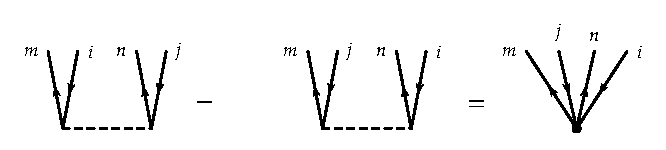
\includegraphics[width=0.75\textwidth]{pictures/8_10}
\par\end{centering}
\caption{\label{fig:8_10}方程 (\ref{eq:rpa_ab_matrices_def}) 中矩阵 $B$ 元素的图形表示。}
\end{figure}

正如观察式 (\ref{eq:rpa_ab_matrices_def}) 中的矩阵 $B$ 所见，除图 8.3 中的图形外，RPA
还包含了\ref{fig:8_10} 中所示的图形，它们具有虚 $2p\text{-}2h$ 激发的物理意义。

\subsection{RPA 的稳定性\label{subsec:8.4.2_RPA=007684=007A33=005B9A=006027}}

矩阵

\begin{equation}
\mathcal{S}=\begin{pmatrix}A & B\\
B^{*} & A^{*}
\end{pmatrix}\label{eq:rpa_stability_matrix_def}
\end{equation}

恰好是在式 (7.37) 中推导出的 HF 理论稳定性矩阵。它是一个 Hermitian 矩阵，其实数本征值表征了 HF 解的物理性质。若
$\mathcal{S}$ 是正定的，则它对应于能量曲面上的极小值点。在这种情况下，我们可以计算矩阵 $\mathcal{S}$
的平方根，并将本征值问题 (\ref{eq:rpa_matrix_equation}) 变换为更对称的形式：

\begin{equation}
\mathcal{S}^{1/2}\eta\mathcal{S}^{1/2}\left(\mathcal{S}^{1/2}\begin{pmatrix}X^{\nu}\\
Y^{\nu}
\end{pmatrix}\right)=\hbar\Omega_{\nu}\left(\mathcal{S}^{1/2}\begin{pmatrix}X^{\nu}\\
Y^{\nu}
\end{pmatrix}\right)\label{eq:rpa_s_half_hermitian}
\end{equation}

其中

\begin{equation}
\eta=\begin{pmatrix}1 & 0\\
0 & -1
\end{pmatrix}\label{eq:rpa_eta_metric_def}
\end{equation}

这是一个仅具有实数本征值的 Hermitian 本征值问题。换言之，若 HF 解对应于能量曲面上的极小值而非鞍点或极大值，则相应的
RPA 方程仅具有实数激发频率［Th 61a］。反之则未必成立。在下文中，我们将假定仅存在实数频率。

\subsection{归一化与完备性关系\label{subsec:8.4.3_=005F52=004E00=005316=004E0E=005B8C=005907=006027=005173=007CFB}}

由于 RPA 矩阵不是 Hermitian 矩阵，其本征矢在通常意义下并不正交。激发态 $|\nu\rangle=Q^{\dagger}_{\nu}|\text{RPA}\rangle$
相互正交的条件给出了正交性关系：

\begin{equation}
\langle\nu|\nu'\rangle=\langle\text{RPA}|[Q_{\nu},Q^{\dagger}_{\nu'}]|\text{RPA}\rangle=\sum_{mi}\left(X^{\nu*}_{mi}X^{\nu'}_{mi}-Y^{\nu*}_{mi}Y^{\nu'}_{mi}\right)=\delta_{\nu\nu'}\label{eq:rpa_orthonormality_condition}
\end{equation}

事实上，我们可以证明 $\nu\ne\nu'$ 的 RPA 方程的解严格满足这一关系。对于 $\nu=\nu'$，若其范数为正，这为我们提供了归一化矢量
$(X^{\nu},Y^{\nu})$ 的准则［Th 61a］。

引入如下矩阵十分便利：

\begin{equation}
\mathcal{X}=\begin{pmatrix}X & Y^{*}\\
Y & X^{*}
\end{pmatrix},\quad\Omega=\begin{pmatrix}\Omega_{\nu} & 0\\
0 & -\Omega_{\nu}
\end{pmatrix}\label{eq:rpa_big_x_matrix_def}
\end{equation}

此时，RPA 方程具有如下紧凑形式：

\begin{equation}
\mathcal{S}\mathcal{X}=\eta\mathcal{X}\hbar\Omega\label{eq:rpa_compact_matrix_form}
\end{equation}

简单的矩阵代数运算表明：

\begin{equation}
[\Omega,\mathcal{X}^{\dagger}\eta\mathcal{X}]=0\label{eq:rpa_commutator_omega_x}
\end{equation}

即 $\Omega$ 与 $\mathcal{X}^{\dagger}\eta\mathcal{X}$ 对易，因此 $\mathcal{X}^{\dagger}\eta\mathcal{X}$
与 $\Omega$ 同时对角化。由于矢量的归一化尚未确定，我们选取：

\begin{equation}
\mathcal{X}^{\dagger}\eta\mathcal{X}=\eta\label{eq:rpa_orthonormality_matrix_form}
\end{equation}

这正是正交归一化条件 (\ref{eq:rpa_orthonormality_condition})。完备性条件则通过将式 (\ref{eq:rpa_orthonormality_matrix_form})
两边乘以 $\eta$ 得到，表明 $\eta\mathcal{X}^{\dagger}$ 是 $\mathcal{X}$ 的逆矩阵：

\begin{equation}
\mathcal{X}\eta\mathcal{X}^{\dagger}=\eta\label{eq:rpa_completeness_matrix_form}
\end{equation}

显式写出即为：

\begin{align}
\sum_{\nu}\left(X^{\nu}_{mi}X^{\nu*}_{nj}-Y^{\nu*}_{mi}Y^{\nu}_{nj}\right) & =\delta_{mn}\delta_{ij},\nonumber \\
\sum_{\nu}\left(X^{\nu}_{mi}Y^{\nu*}_{nj}-Y^{\nu*}_{mi}X^{\nu}_{nj}\right) & =0\label{eq:rpa_closure_explicit}
\end{align}


\subsection{RPA 方程的数值求解\label{subsec:8.4.4_RPA=0065B9=007A0B=007684=006570=00503C=006C42=0089E3}}

在许多实际问题中，RPA 矩阵 $A$ 和 $B$ 均为实数。对于实频率 $\Omega_{\nu}$，求解问题可以简化为对角化一个维度仅为原维度一半的实对称矩阵。

我们定义矢量：

\begin{equation}
P^{\nu}=\frac{\mathrm{i}}{\sqrt{2}}(X^{\nu}+Y^{\nu}),\quad Q^{\nu}=\frac{1}{\sqrt{2}}(X^{\nu}-Y^{\nu})\label{eq:rpa_pq_vectors_def}
\end{equation}

由式 (\ref{eq:rpa_matrix_equation}) 容易推得：

\begin{align}
\mathrm{i}(A-B)Q^{\nu} & =\hbar\Omega_{\nu}P^{\nu},\nonumber \\
-\mathrm{i}(A+B)P^{\nu} & =\hbar\Omega_{\nu}Q^{\nu}\label{eq:rpa_pq_decoupled_system}
\end{align}

从而：

\begin{equation}
(A+B)(A-B)Q^{\nu}=\hbar^{2}\Omega^{2}_{\nu}Q^{\nu}\label{eq:rpa_squared_frequency_problem}
\end{equation}

伴随着稳定性矩阵 $\mathcal{S}$ 的正定性，矩阵 $(A\pm B)$ 同样正定。我们可以利用 Cholesky 分解将
$A-B$ 分解为下三角矩阵及其转置的乘积：

\begin{equation}
A-B=LL^{T}\label{eq:rpa_cholesky_decomposition}
\end{equation}

进而将求解转化为实对称本征值问题：

\begin{equation}
L^{T}(A+B)LR^{\nu}=\hbar^{2}\Omega^{2}_{\nu}R^{\nu}\label{eq:rpa_symmetric_eigenproblem}
\end{equation}

求出本征值 $\hbar\Omega_{\nu}$ 与正交归一本征矢 $R^{\nu}$ 后，便可恢复出正确归一化的 RPA 振幅
$X^{\nu}$ 和 $Y^{\nu}$。

\subsection{玻色子算符表象\label{subsec:8.4.5_=0073BB=008272=005B50=007B97=007B26=008868=008C61}}

在推导 RPA 方程 (\ref{eq:rpa_matrix_equation}) 时，我们采用了准玻色子近似 (\ref{eq:rpa_quasiboson_commutation})，即用玻色子算符
$B_{mi}$ 替代 ph 算符 $a^{\dagger}_{m}a_{i}$：

\begin{equation}
a^{\dagger}_{m}a_{i}\to B^{\dagger}_{mi},\quad a^{\dagger}_{i}a_{m}\to B_{mi}\label{eq:rpa_boson_mapping}
\end{equation}

它们满足严格的玻色子对易关系：

\begin{equation}
[B_{mi},B^{\dagger}_{nj}]=\delta_{mn}\delta_{ij},\quad[B_{mi},B_{nj}]=0\label{eq:rpa_boson_commutation_exact}
\end{equation}

在此表象下，保留至简谐阶次的玻色子 Hamiltonian 量为：

\begin{equation}
H_{B}=E_{\text{HF}}-\frac{1}{2}\operatorname{Tr}A+\frac{1}{2}\begin{pmatrix}B^{\dagger} & B\end{pmatrix}\begin{pmatrix}A & B\\
B^{*} & A^{*}
\end{pmatrix}\begin{pmatrix}B\\
B^{\dagger}
\end{pmatrix}\label{eq:rpa_boson_hamiltonian}
\end{equation}

通过引入玻色子 Bogoliubov 变换：

\begin{equation}
O^{\dagger}_{\nu}=\sum_{mi}\left(X^{\nu}_{mi}B^{\dagger}_{mi}-Y^{\nu}_{mi}B_{mi}\right)\label{eq:rpa_boson_bogoliubov}
\end{equation}

Hamiltonian 量 (\ref{eq:rpa_boson_hamiltonian}) 可被完全对角化为独立简谐振子的集合：

\begin{equation}
H_{B}=E_{\text{RPA}}+\sum_{\nu>0}\hbar\Omega_{\nu}O^{\dagger}_{\nu}O_{\nu}\label{eq:rpa_diagonal_boson_h}
\end{equation}

式中 RPA 基态能为：

\begin{equation}
E_{\text{RPA}}=E_{\text{HF}}-\sum_{\nu>0}\hbar\Omega_{\nu}\operatorname{Tr}(Y^{\nu\dagger}Y^{\nu})=E_{\text{HF}}-\frac{1}{2}\sum_{\nu>0}\left(E^{\text{TDA}}_{\nu}-\hbar\Omega_{\nu}\right)\label{eq:rpa_ground_energy_lowering}
\end{equation}

这表明由于基态关联的存在，RPA 基态能相对于 Hartree-Fock 基态能有所降低，其降低量恰好等于 RPA 与 TDA 各激发能之差总和的一半。

\subsection{RPA 基态的构造\label{subsec:8.4.6_RPA=0057FA=006001=007684=006784=009020}}

RPA 基态最初由式 (\ref{eq:rpa_vacuum_condition}) 定义为算符 $Q_{\nu}$ 的真空。在准玻色子近似下，它等价于玻色子算符
$O_{\nu}$ 的真空 $|\text{RPA}\rangle$：

\begin{equation}
O_{\nu}|\text{RPA}\rangle=0\label{eq:rpa_boson_vacuum_condition}
\end{equation}

类比于第 7 章利用准粒子 Thouless 定理构造真空的做法，我们可以通过 Thouless 定理［Th 60］从玻色子 $B_{mi}$
的真空 $|\text{HF}\rangle$ 显式构造出 RPA 基态：

\begin{equation}
|\text{RPA}\rangle=N_{0}\exp\left(\frac{1}{2}\sum_{minj}Z_{minj}B^{\dagger}_{mi}B^{\dagger}_{nj}\right)|\text{HF}\rangle\label{eq:rpa_thouless_ground_state}
\end{equation}

其中 $N_{0}$ 为归一化系数，且：

\begin{equation}
Z=Y^{*}X^{*-1}\label{eq:rpa_thouless_z_matrix}
\end{equation}

式 (\ref{eq:rpa_thouless_ground_state}) 表明，RPA 基态波函数包含了 $2p\text{-}2h,4p\text{-}4h,\dots$
等任意偶数粒子-空穴对的相干关联。

\subsection{不变性与赝解\label{subsec:8.4.7_=004E0D=0053D8=006027=004E0E=008D5D=0089E3}}

在下文中，我们假设精确的两体 Hamiltonian 量 $H$ 在由 Hermitian 单体算符 $P$ 所生成的连续对称操作下是不变的（例如全核质心平移的情况）；并进一步假定
HF 解破坏了该对称性。这特别意味着 HF 单粒子密度 $\rho^{(0)}$ 与 $P$ 不对易：

\begin{equation}
[\rho^{(0)},P]\ne0\label{eq:rpa_broken_symmetry_condition}
\end{equation}

由于 $\rho^{(0)}$ 在 HF 基下是对角的（对粒子能级为 0，对空穴能级为 1），这表明并非所有 ph 矩阵元 $P_{mi}$
都为零。由于精确 Hamiltonian 量与 $P$ 对易：

\begin{equation}
[H,P]=0\label{eq:rpa_exact_commutation_hp}
\end{equation}

因此 $P$ 是 RPA 方程的一个精确但属于赝模的解：

\begin{equation}
\begin{pmatrix}A & B\\
B^{*} & A^{*}
\end{pmatrix}\begin{pmatrix}P\\
-P^{*}
\end{pmatrix}=0\label{eq:rpa_spurious_zero_mode}
\end{equation}

式中 $P$ 为粒子-空穴空间中的矢量 $P_{mi}$。相应的态为：

\begin{equation}
P|\text{HF}\rangle=\sum_{mi}\left(P_{mi}a^{\dagger}_{m}a_{i}+P^{*}_{mi}a^{\dagger}_{i}a_{m}\right)|\text{HF}\rangle\label{eq:rpa_spurious_state_vector}
\end{equation}

我们认识到，RPA 方程 (\ref{eq:rpa_matrix_equation}) 仅在 HF 解确实破缺了该对称性时才具有此类解；否则矩阵元
$P_{mi}$ 恒等于零。

因此我们看到：只要我们在 RPA 中进行精确计算并采用自洽的单粒子能与波函数，对应于 HF 态中破缺对称性的赝激发（例如原子核作为整体的平移运动）就会完全自动解耦分离出来。它们与所有其他物理激发严格正交，且其激发能严格位于零能量处。这是
RPA 相比于 TDA 的重大优势所在，在 TDA 中赝解与真实物理态会发生严重的非物理混合。

为了求解与该零模共轭的正规坐标 $Q_{0}$，我们根据 Thouless 和 Valatin［TV 62］的方法建立非齐次方程组：

\begin{equation}
\begin{pmatrix}A & B\\
B^{*} & A^{*}
\end{pmatrix}\begin{pmatrix}Q_{0}\\
Q^{*}_{0}
\end{pmatrix}=\frac{\hbar}{\mathrm{i}M_{0}}\begin{pmatrix}P_{0}\\
-P^{*}_{0}
\end{pmatrix}\label{eq:rpa_thouless_valatin_eq}
\end{equation}

结合对易关系 $[Q_{0},P_{0}]=\mathrm{i}\hbar$，便可确定惯量参数 $M_{0}$。此时玻色子 Hamiltonian
量在零模与内禀振动之间完全解耦：

\begin{equation}
H_{B}=E_{\text{RPA}}+\frac{1}{2M_{0}}P^{2}_{0}+\sum_{\nu>0}\hbar\Omega_{\nu}O^{\dagger}_{\nu}O_{\nu}\label{eq:rpa_hamiltonian_with_zero_mode}
\end{equation}

对于平移运动，$M_{0}$ 恰为总核质量 $Am$；对于转动运动，$M_{0}$ 恰为著名的 Thouless-Valatin
转动惯量 $\mathcal{J}_{\text{TV}}$。

\section{线性响应理论\label{sec:8.5_=007EBF=006027=0054CD=005E94=007406=008BBA}}

在计算核系统的集体激发时，迄今为止我们均采用了定态 Schrödinger 方程 (\ref{eq:rpa_exact_eigenstates})，并尝试至少在某种近似下对角化
Hamiltonian 量。

现在我们将从一个截然不同的出发点展开研究。我们考查外加含时外场：

\begin{equation}
F(t)=Fe^{-\mathrm{i}\omega t}+F^{\dagger}e^{\mathrm{i}\omega t}\label{eq:linresp_external_field}
\end{equation}

对核系统的影响。我们假设 $F$ 是单体算符，且外场足够微弱，即它仅引起核密度的微小改变，使我们能够在满意的精度下在线性阶次内进行处理。

正如我们将看到的，核密度将随着该外场发生振荡；且每当外场频率 $\omega$ 接近系统的某一激发能量时，就会产生共振。通过这种途径：
\begin{enumerate}
\item 我们能够获取关于系统激发态的信息。特别地，我们找到了决定振幅 $\langle0|a^{\dagger}_{i}a_{m}|\nu\rangle$
的方程，它精确地对应于 RPA 方程。
\item 我们能够计算系统对外场的响应，即其密度、能量等物理量的动态改变。
\item 我们找到了一种为密度依赖相互作用推导 RPA 方程的普适方法。
\end{enumerate}

\subsection{线性响应方程的推导\label{subsec:8.5.1_=007EBF=006027=0054CD=005E94=0065B9=007A0B=007684=0063A8=005BFC}}

处于外加含时场中的核系统的波函数 $|\Phi(t)\rangle$ 不再是定态。它是一个波包，其单体密度：

\begin{equation}
\rho_{kk'}(t)=\langle\Phi(t)|a^{\dagger}_{k'}a_{k}|\Phi(t)\rangle\label{eq:linresp_density_matrix_def}
\end{equation}

此时显式地依赖于时间。我们希望在以下近似下显式计算该密度：
\begin{enumerate}
\item 我们假设在任何时刻 $\rho(t)$ 均对应于一个 Slater 行列式\footnote{即 $\rho^{2}=\rho$。在此意义下，以下对 RPA 的推导表明它正是独立粒子图像的含时推广（参见第 12 章）。}。此时
$\rho$ 服从如下运动方程：
\end{enumerate}
\begin{equation}
\mathrm{i}\hbar\dot{\rho}=[h[\rho]+f(t),\rho]\label{eq:linresp_tdhf_eom}
\end{equation}

这正是时间相关 Hartree-Fock（TDHF）方程。它将在第 12.2 节中详细推导。在此 $h[\rho]$ 是式 (5.33)
定义的单粒子 Hartree-Fock 场，而 $f(t)$ 是式 (\ref{eq:linresp_external_field})
的含时外场。
\begin{enumerate}
\item 我们假设外场 $f(t)$ 是微弱的，即它仅引起围绕定常密度 $\rho^{(0)}$ 的小振幅振荡，而 $\rho^{(0)}$
本身是定态 Hartree-Fock 方程 $[h[\rho^{(0)}],\rho^{(0)}]=0$ 的自洽解。因此，密度具有如下形式：
\end{enumerate}
\begin{equation}
\rho(t)=\rho^{(0)}+\delta\rho(t)\label{eq:linresp_density_split}
\end{equation}

其中

\begin{equation}
\delta\rho(t)=\rho^{(1)}e^{-\mathrm{i}\omega t}+\rho^{(1)\dagger}e^{\mathrm{i}\omega t}\label{eq:linresp_deltarho_fourier}
\end{equation}

线性地依赖于外场 $f$。在下文中，我们在使 $\rho^{(0)}$ 与 $h[\rho^{(0)}]$ 同时对角化的基矢——即自洽
HF 单粒子基——下开展讨论：

\begin{align}
\rho^{(0)}_{kk'} & =\delta_{kk'}\times\begin{cases}
1, & \text{对空穴能级},\\
0, & \text{对粒子能级},
\end{cases}\label{eq:linresp_rho0_diagonal}\\
(h_{0})_{kk'} & =(h[\rho^{(0)}])_{kk'}=\delta_{kk'}\epsilon_{k}\label{eq:linresp_h0_diagonal}
\end{align}

将式 (\ref{eq:linresp_density_split}) 代入 TDHF 方程 (\ref{eq:linresp_tdhf_eom})
并展开至外场 $f$ 的一阶线性项，得到：

\begin{equation}
\mathrm{i}\hbar\delta\dot{\rho}=[h_{0},\delta\rho]+\left[\frac{\delta h}{\delta\rho}\cdot\delta\rho,\rho^{(0)}\right]+[f(t),\rho^{(0)}]\label{eq:linresp_linearized_eom}
\end{equation}

式中 $\frac{\delta h}{\delta\rho}\cdot\delta\rho$ 是对下式的简写：

\begin{equation}
\left(\frac{\delta h}{\delta\rho}\cdot\delta\rho\right)_{kk'}=\sum_{ll'}\frac{\delta h_{kk'}}{\delta\rho_{ll'}}\delta\rho_{ll'}\label{eq:linresp_deltah_chain}
\end{equation}

利用 Slater 行列式条件 $\rho^{2}=\rho$ 导出的关系 $\rho^{(0)}\delta\rho+\delta\rho\rho^{(0)}=\delta\rho$，可以证明
$\delta\rho$ 仅具有粒子-空穴（ph）与空穴-粒子（hp）矩阵元。将式 (\ref{eq:linresp_linearized_eom})
投影到 ph 与 hp 基上，便得到线性响应方程组：

\begin{equation}
\begin{pmatrix}A-\hbar\omega & B\\
B^{*} & A^{*}+\hbar\omega
\end{pmatrix}\begin{pmatrix}\rho^{(1)}_{mi}\\
\rho^{(1)}_{im}
\end{pmatrix}=-\begin{pmatrix}f_{mi}\\
f_{im}
\end{pmatrix}\label{eq:linresp_matrix_system}
\end{equation}

式中矩阵 $A$ 与 $B$ 定义为：

\begin{align}
A_{minj} & =(\epsilon_{m}-\epsilon_{i})\delta_{mn}\delta_{ij}+\frac{\delta h_{mi}}{\delta\rho_{nj}},\nonumber \\
B_{minj} & =\frac{\delta h_{mi}}{\delta\rho_{jn}}\label{eq:linresp_ab_functional_derivative}
\end{align}

对于密度无关的两体相互作用，式 (\ref{eq:linresp_ab_functional_derivative}) 精确地退化为我们在第
8.4.1 节式 (\ref{eq:rpa_ab_matrices_def}) 中定义的矩阵元。然而，式 (\ref{eq:linresp_ab_functional_derivative})
的深远意义在于它同样适用于任何密度依赖的有效力（例如 Skyrme 力或 Gogny 力），此时剩余相互作用由能量泛函对密度的二阶泛函微商给出。

将式 (\ref{eq:linresp_matrix_system}) 形式求逆，可将系统的动态响应写为响应函数（极化传播子）$R(\omega)$
的作用：

\begin{equation}
\rho^{(1)}_{pq}=\sum_{p'q'}R_{pq,p'q'}(\omega)f_{p'q'}\label{eq:linresp_response_function_action}
\end{equation}

在零外场（$f=0$）下，式 (\ref{eq:linresp_matrix_system}) 的齐次方程恰好对应于响应函数 $R(\omega)$
的极点条件 $\omega=\Omega_{\nu}$：

\begin{equation}
\begin{pmatrix}A & B\\
B^{*} & A^{*}
\end{pmatrix}\begin{pmatrix}X^{\nu}\\
Y^{\nu}
\end{pmatrix}=\hbar\Omega_{\nu}\begin{pmatrix}1 & 0\\
0 & -1
\end{pmatrix}\begin{pmatrix}X^{\nu}\\
Y^{\nu}
\end{pmatrix}\label{eq:linresp_rpa_eigen_recovered}
\end{equation}

这正是 RPA 方程！它证明了：RPA 近似本质上就是含时平均场理论的小振幅极限。

借助 RPA 的完整本征解集，响应函数 $R(\omega)$ 可显式写为其谱表象（Lehmann 表象）：

\begin{equation}
R_{pq,p'q'}(\omega)=\sum_{\nu>0}\left[\frac{\rho^{(\nu)}_{pq}\rho^{(\nu)*}_{p'q'}}{\hbar(\omega-\Omega_{\nu}+\mathrm{i}\eta)}-\frac{\rho^{(\nu)*}_{qp}\rho^{(\nu)}_{q'p'}}{\hbar(\omega+\Omega_{\nu}+\mathrm{i}\eta)}\right]\label{eq:linresp_spectral_representation}
\end{equation}

它服从著名的 Bethe-Salpeter 方程：

\begin{equation}
R(\omega)=R^{0}(\omega)+R^{0}(\omega)\bar{v}R(\omega)\label{eq:linresp_bethe_salpeter}
\end{equation}

式中 $R^{0}(\omega)$ 为无剩余相互作用时的自由响应函数（独立粒子响应函数）。

\subsection{激发几率的计算与示意模型\label{subsec:8.5.2_=006FC0=0053D1=0051E0=007387=007684=008BA1=007B97=004E0E=00793A=00610F=006A21=00578B}}

在示意模型中，剩余相互作用采用可分离形式 $\bar{v}_{mjin}=\chi D_{mi}D^{*}_{nj}$［式 (\ref{eq:tda_separable_force})］，此时由式
(\ref{eq:linresp_bethe_salpeter}) 容易导出如下色散关系：

\begin{equation}
\frac{1}{\chi}=R^{0}_{D}(\Omega_{\nu})=\sum_{mi}|D_{mi}|^{2}\frac{2\epsilon_{mi}}{\hbar^{2}\Omega^{2}_{\nu}-\epsilon^{2}_{mi}}\label{eq:linresp_schematic_dispersion}
\end{equation}

\begin{figure}[H]
\begin{centering}
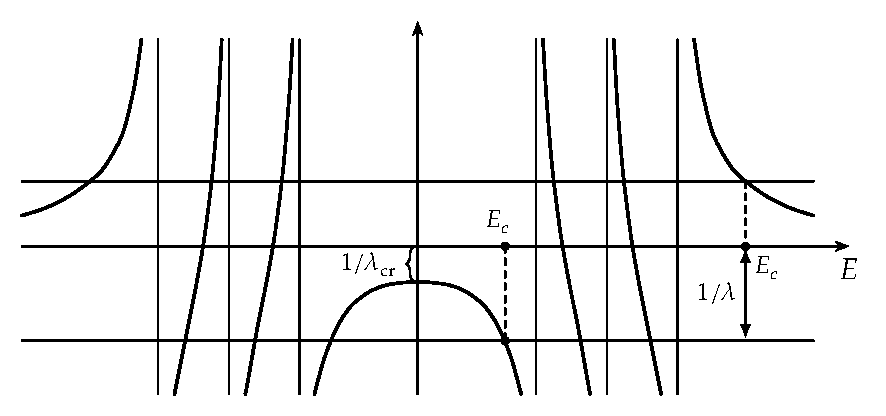
\includegraphics[width=0.75\textwidth]{pictures/8_11}
\par\end{centering}
\caption{\label{fig:8_11}色散关系 (\ref{eq:linresp_schematic_dispersion}) 的图解。}
\end{figure}

方程 (\ref{eq:linresp_schematic_dispersion}) 可以通过与 TDA 情形相同的方式在图形上求解。对比\ref{fig:8_11}
与图 8.4，我们可以注意到源于 RPA 基态关联的两个质的差异：
\begin{enumerate}
\item 当剩余相互作用强于某一临界值（即 $\chi<\chi_{\text{crit}}$）时，低激发集体态的能量变为纯虚数，标志着球形基态对形变破缺发生失稳。
\item 对于可比的相互作用强度 $\chi$，$T=0$ 的 RPA 集体态比对应的 TDA 态被向下拉得更低。
\end{enumerate}
在简并情形（所有 $\epsilon_{mi}=\epsilon$）下，集体态能量显式给出为：

\begin{equation}
E^{2}_{\text{coll}}=\hbar^{2}\Omega^{2}_{\text{coll}}=\epsilon^{2}+2\epsilon\chi\sum_{mi}|D_{mi}|^{2}\label{eq:linresp_degenerate_energy_squared}
\end{equation}

临界耦合强度为：

\begin{equation}
\chi_{\text{crit}}=-\frac{\epsilon}{2\sum_{mi}|D_{mi}|^{2}}\label{eq:linresp_critical_coupling}
\end{equation}

这正是球形 HF 解不再对应能量极小值的点，系统在此处发生从球形相到形变相的相变。在 TDA 中，相应的相变直到 $2\chi_{\text{crit}}$
处才发生。

计算响应函数 $R_{D}(\omega)$ 在极点 $\omega=\Omega_{\nu}$ 处的留数，给出到集体态的跃迁几率：

\begin{equation}
|\langle\nu|D|0\rangle|^{2}=\frac{\epsilon}{E_{\text{coll}}}\sum_{mi}|D_{mi}|^{2}\label{eq:linresp_enhanced_transition_prob}
\end{equation}

可以看到，对于低激发集体态，跃迁几率相比于 TDA 结果 (\ref{eq:tda_collective_transition_prob})
进一步放大了 $\epsilon/E_{\text{coll}}$ 倍。对于低激发的集体八极和四极态，该增强因子可高达 2 左右。

\subsection{静态极化率与转动惯量\label{subsec:8.5.3_=009759=006001=006781=005316=007387=004E0E=008F6C=0052A8=0060EF=0091CF}}

我们可以应用线性响应理论计算核系统在静态外场 $-\lambda F$ 下的能量改变与形变。这相当于在线性响应理论中求解受约束 Hartree-Fock（CHF）方程：

\begin{equation}
\delta\langle\Phi|H-\lambda F|\Phi\rangle=0\label{eq:linresp_chf_equation}
\end{equation}

由式 (\ref{eq:linresp_matrix_system})，零频极限下的密度改变量为：

\begin{equation}
\rho^{(1)}=\lambda\mathcal{S}^{-1}f\label{eq:linresp_static_density_response}
\end{equation}

静态极化率 $\alpha$ 定义为算符 $F$ 的期望值变化：

\begin{equation}
\delta\langle F\rangle=\operatorname{Tr}(F\delta\rho)=\alpha\lambda\label{eq:linresp_polarizability_def}
\end{equation}

体系能量的相应改变为：

\begin{equation}
\delta E=-\frac{1}{2}\alpha\lambda^{2}\label{eq:linresp_energy_second_order}
\end{equation}

由能量曲面在极小值点 $\lambda=0$ 处的曲率，我们得到静态极化率：

\begin{equation}
\alpha=\frac{\mathrm{d}^{2}E}{\mathrm{d}\lambda^{2}}=f^{\dagger}\mathcal{S}^{-1}f=2\sum_{\nu>0}\frac{|\langle\nu|F|0\rangle|^{2}}{\hbar\Omega_{\nu}}\label{eq:linresp_polarizability_sum_rule}
\end{equation}

这表明静态极化率与反能量加权求和规则 $S_{-1}$ 紧密联系在一起。

将上述形式体系应用于自洽推转模型（cranking model，参见第 7.7 节），外加约束场为推转算符 $\omega J_{x}$。线性响应方程即给出著名的
Thouless-Valatin 方程：

\begin{equation}
\mathcal{S}\delta\rho^{(1)}=\omega J_{x}\label{eq:linresp_tv_cranking_eq}
\end{equation}

进而给出完整的 Thouless-Valatin 自洽微观转动惯量：

\begin{equation}
\mathcal{J}_{\text{TV}}=\frac{\mathrm{d}^{2}E}{\mathrm{d}\omega^{2}}=2\sum_{\nu>0}\frac{|\langle\nu|J_{x}|0\rangle|^{2}}{\hbar\Omega_{\nu}}\label{eq:linresp_thouless_valatin_inertia}
\end{equation}


\subsection{连续谱中的 RPA 方程\label{subsec:8.5.4_=008FDE=007EED=008C31=004E2D=007684RPA=0065B9=007A0B}}

在实际的原子核巨共振激发中，单粒子能量通常高于粒子分离阈，核子可以发射到连续谱中。因此，真实问题并非离散的束缚态本征值问题，而是具有连续能量本征值的散射与共振问题。物理上关心的核心量是跃迁强度函数：

\begin{equation}
S_{F}(\omega)=\sum_{\nu>0}|\langle\nu|F|0\rangle|^{2}\delta(\hbar\omega-\hbar\Omega_{\nu})=-\frac{1}{\pi}\operatorname{Im}R_{F}(\omega)\label{eq:linresp_strength_function_im_r}
\end{equation}

巨共振在连续谱中的物理宽度源于两个截然不同的物理机制：
\begin{enumerate}
\item 衰变宽度（出射宽度，decay width $\Gamma^{\uparrow}$）：波函数中的单粒子分量处于 HF 势的连续散射态上，核子可以直接隧穿逸出衰变为自由粒子和
$A-1$ 核的空穴态。
\item 展宽宽度（扩散宽度，spreading width $\Gamma^{\downarrow}$）：ph 激发组态与更为复杂的 $2p\text{-}2h$
及更高级复合核组态相耦合，使跃迁强度弥散在密集的背景态之中。
\end{enumerate}
对于具有零力程相互作用（例如 Skyrme 力）的核系统，Bertsch、Tsai、Shlomo、Liu 等人［Be 73, SB
75, BT 75, LG 76b］发展了在坐标空间中求解 Bethe-Salpeter 方程的强大技术。引入单粒子 Green 函数：

\begin{equation}
G(\boldsymbol{r},\boldsymbol{r}',\omega)=\langle\boldsymbol{r}|\frac{1}{\hbar\omega-h_{0}+\mathrm{i}\eta}|\boldsymbol{r}'\rangle=-\frac{2m}{\hbar^{2}}\sum_{ljm}\frac{v_{lj}(r_{<})w_{lj}(r_{>})}{W(v,w)}Y_{ljm}(\hat{\boldsymbol{r}})Y^{*}_{ljm}(\hat{\boldsymbol{r}}')\label{eq:linresp_single_particle_green}
\end{equation}

其中 $v(r)$ 与 $w(r)$ 分别为在原点正则与在无穷远满足出射波边界条件的两个线性无关单粒子解，$W(v,w)$ 为其
Wronskian 决定式。无相互作用响应函数 $R^{0}(\boldsymbol{r},\boldsymbol{r}',\omega)$
即可闭合表达为束缚空穴波函数与该 Green 函数的折积：

\begin{equation}
R^{0}(\boldsymbol{r},\boldsymbol{r}',\omega)=\sum_{i}\left[\phi^{*}_{i}(\boldsymbol{r})\phi_{i}(\boldsymbol{r}')G(\boldsymbol{r},\boldsymbol{r}',\epsilon_{i}+\hbar\omega)+\phi_{i}(\boldsymbol{r})\phi^{*}_{i}(\boldsymbol{r}')G(\boldsymbol{r}',\boldsymbol{r},\epsilon_{i}-\hbar\omega)\right]\label{eq:linresp_r0_coordinate_space}
\end{equation}

在此基础上，全响应函数满足坐标空间一维积分方程：

\begin{equation}
R(\boldsymbol{r},\boldsymbol{r}',\omega)=R^{0}(\boldsymbol{r},\boldsymbol{r}',\omega)+V_{0}\int\mathrm{d}^{3}r''R^{0}(\boldsymbol{r},\boldsymbol{r}'',\omega)R(\boldsymbol{r}'',\boldsymbol{r}',\omega)\label{eq:linresp_coordinate_bethe_salpeter}
\end{equation}

利用球谐函数展开将角向坐标积出后，式 (\ref{eq:linresp_coordinate_bethe_salpeter}) 化为径向坐标网格点上的非齐次代数线性方程组，其数值求解极为高效，且严格精确地包含了连续谱边界条件。

\section{应用及与实验的比较\label{sec:8.6_=005E94=007528=0053CA=004E0E=005B9E=009A8C=007684=006BD4=008F83}}

\subsection{唯象基下的粒子-空穴计算\label{subsec:8.6.1_=00552F=008C61=0057FA=004E0B=007684=007C92=005B50-=007A7A=007A74=008BA1=007B97}}

早在 1957 年，Elliott 和 Flowers［EF 57］就针对双幻核 $^{16}\mathrm{O}$ 的负宇称态进行了开创性的
TDA 计算。他们采用了谐振子基，组态空间包含用于 $1^{-}$ 通道的 5 个 ph 态以及用于 $3^{-}$ 通道的 3
个 ph 态。采用带有 Rosenfeld 交换混合的 Yukawa 相互作用［EF 57, 表 4.3］，他们发现在约 $7\,\text{MeV}$
处存在一个高度集体的 $3^{-},\,T=0$ 态，以及在 $22.6\,\text{MeV}$ 和 $25.2\,\text{MeV}$
处的两个集体 $1^{-},\,T=1$ 态。在该组态空间中，八极态耗尽了 68\% 的 $S_{0}$ 求和规则，两个偶极态耗尽了
97\% 的求和规则。这在定性上与示意模型（第 8.2.2 节）的结果完全一致。跃迁强度主要集中在从无微扰单粒子能量（约 $11.5\,\text{MeV}$）显著移开的一个能级上。

Gillet 等人［Gi 64, GV 64, GS 64, GGS 66］通过在闭壳核 $^{12}\mathrm{C}$、$^{16}\mathrm{O}$、$^{40}\mathrm{Ca}$
和 $^{208}\mathrm{Pb}$ 中对比 TDA 与 RPA 计算，系统研究了基态关联的影响。他们发现，对于 $T=1$
能级，RPA 的结果与 TDA 相比变化不大；然而低激发的 $T=0$ 态在 RPA 中得到了好得多的重现。特别是 RPA 的激发几率显著大于
TDA 的值。

Ring 和 Speth［RS 74a］应用了由 Migdal［Mi 67］发展的有限费米系统理论。该理论从截然不同的视角出发，用短程且依赖于密度的重整化有效相互作用［式
(4.113)］来描述准粒子与准空穴之间的相互作用，并以计算集体态的 RPA 方程告终。在铅同位素区域［RS 73, RS 74a］，他们采用
Woods-Saxon 基展开、包含费米面上下各两个主壳的大组态空间，计算了 $^{208}\mathrm{Pb}$ 的低激发态能谱与跃迁几率，列于表
8.1 中。

\begin{table}[H]
\caption{\label{tab:8_1}基于 Migdal 力在 RPA 理论下计算得到的 $^{208}\mathrm{Pb}$ 低激发集体态的能量与激发几率［RS
74a］。}

\centering{}%
\begin{tabular}{cccccc}
\hline 
$I^{\pi}$ & \multicolumn{2}{c}{$E(I)\,[\text{MeV}]$} & \multicolumn{2}{c}{$B(E/M)I$} & 单位\tabularnewline
\hline 
 & 理论 & 实验 & 理论 & 实验 & \tabularnewline
\hline 
$3^{-}$ & 2.63 & 2.61 & 546 & $(540\pm30)\times10^{3}$ & $e^{2}\,\text{fm}^{6}$\tabularnewline
$5^{-}$ & 3.39 & 3.19 & 285 & $(462\pm55)\times10^{6}$ & $e^{2}\,\text{fm}^{10}$\tabularnewline
$5^{-}$ & 3.82 & 3.71 & 301 & $330\times10^{6}$ & $e^{2}\,\text{fm}^{10}$\tabularnewline
$2^{+}$ & 4.49 & 4.07 & 3070 & 2965 & $e^{2}\,\text{fm}^{4}$\tabularnewline
$4^{+}$ & 4.69 & 4.32 & 757 & $1287\times10^{4}$ & $e^{2}\,\text{fm}^{8}$\tabularnewline
$6^{+}$ & 4.77 & 4.42 & 210 & $230\times10^{8}$ & $e^{2}\,\text{fm}^{12}$\tabularnewline
$1^{+}$ & 7.50 & 7.56 & 568 & 5.9 & $\mu^{2}_{N}$\tabularnewline
$1^{+}$ & 8.30 & 7.99 & 11.00 & 10.0 & $\mu^{2}_{N}$\tabularnewline
$2^{-}$ & 7.51 & — & $11.00\times10^{3}$ & — & $\mu^{2}_{N}\,\text{fm}^{2}$\tabularnewline
\hline 
\end{tabular}
\end{table}

\begin{figure}[H]
\begin{centering}
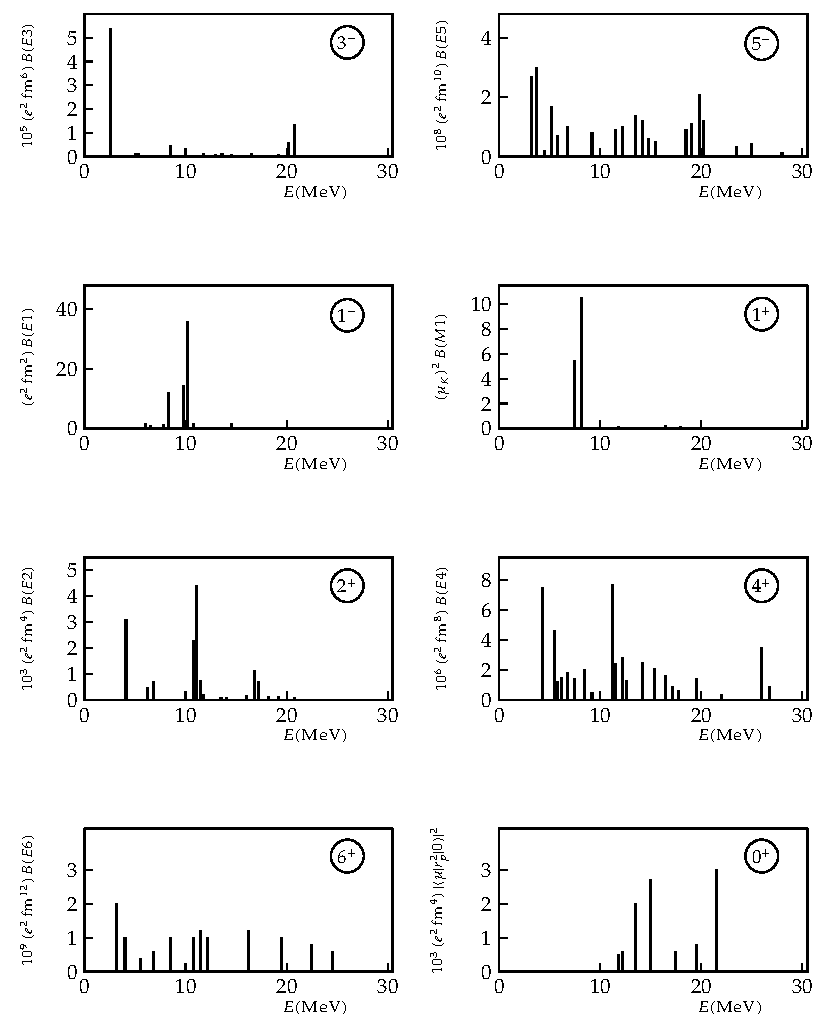
\includegraphics[width=0.8\textwidth]{pictures/8_12}
\par\end{centering}
\caption{\label{fig:8_12}$^{208}\mathrm{Pb}$ 中多极跃迁强度的分布（引自 \cite{RS74a}）。}
\end{figure}

\ref{fig:8_12} 展示了强度的分布情况。特别是，它不仅展示了低激发的 $3^{-},2^{+},4^{+},6^{+}$
集体态，还展示了巨共振，如 $1^{-}$（其能量略微偏低）、$2^{+}$（分裂为 $T=0$ 部分和 $T=1$ 部分）、位于约
$14\,\text{MeV}$ 处的呼吸模（$0^{+}$）以及更高极次的共振。

\subsection{自洽基下的粒子-空穴计算\label{subsec:8.6.2_=0081EA=006D3D=0057FA=004E0B=007684=007C92=005B50-=007A7A=007A74=008BA1=007B97}}

正如我们在第 5 章所见，采用唯象密度依赖有效力（如 Skyrme 力）的 Hartree-Fock 理论能够极好地重现基态性质。在自洽基下，RPA
的剩余相互作用由总能量泛函对密度的二阶泛函微商给出。近年来，Bertsch 等人［BT 75, LB 76, BGG 76, KKS
77］将该自洽理念应用于连续谱 RPA 计算中。

\begin{figure}[H]
\begin{centering}
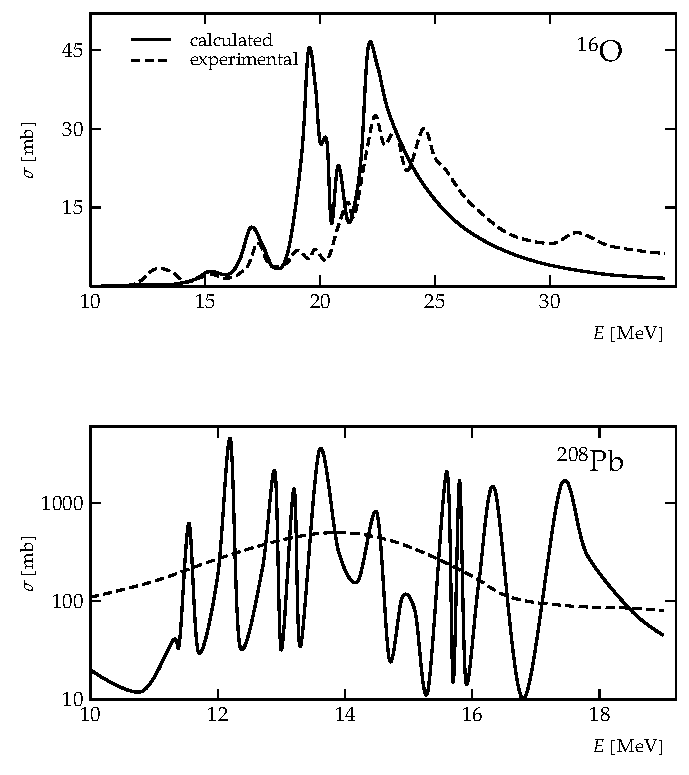
\includegraphics[width=0.8\textwidth]{pictures/8_13}
\par\end{centering}
\caption{\label{fig:8_13}基于连续谱 RPA 计算得到的 $^{16}\mathrm{O}$ 与 $^{208}\mathrm{Pb}$
巨偶极共振光吸收截面。虚线对应于实验值（引自 \cite{LG76b}）。}
\end{figure}

在\ref{fig:8_13} 中，我们看到连续谱 RPA 能够直接计算出巨偶极共振的线宽与出射谱。然而，理论曲线在 $^{208}\mathrm{Pb}$
中呈现出许多尖锐的共振峰，这是由于目前的 RPA 计算仅包含了出射宽度 $\Gamma^{\uparrow}$，未包含源于与 $2p\text{-}2h$
等复杂组态耦合引起的扩散宽度 $\Gamma^{\downarrow}$。

\section{求和规则\label{sec:8.7_=006C42=00548C=0089C4=005219}}

\subsection{强度函数的能量加权矩\label{subsec:8.7.1_=005F3A=005EA6=0051FD=006570=007684=0080FD=0091CF=0052A0=006743=0077E9}}

对于厄米单体算符 $F=\sum_{p}f(\boldsymbol{r}_{p})$，求和规则定义为强度分布的 $k$ 阶矩：

\begin{equation}
S_{k}(F)=\sum_{\nu>0}(E_{\nu}-E_{0})^{k}|\langle\nu|F|0\rangle|^{2}\label{eq:sumrule_moment_def}
\end{equation}

利用完备性关系，可写为：

\begin{equation}
S_{k}=\langle0|F(H-E_{0})^{k}F|0\rangle\label{eq:sumrule_operator_moment}
\end{equation}

根据 Lane 等人［MBF 76, BML 76, BLM 79］的研究，可以定义表征强度分布的特征能量：

\begin{equation}
\bar{E}_{k}=\sqrt{\frac{S_{k}}{S_{k-2}}}\label{eq:sumrule_average_energy_def}
\end{equation}

由 Schwarz 不等式 $S_{k+2}S_{k}\ge S^{2}_{k+1}$，可以导出 $\bar{E}_{3}\ge\bar{E}_{1}$，并且围绕平均能量的均方涨落满足：

\begin{equation}
\sigma^{2}=\bar{E}^{2}-\bar{E}^{2}_{1}\le\frac{1}{4}\left(\bar{E}^{2}_{3}-\bar{E}^{2}_{1}\right)\label{eq:sumrule_energy_dispersion_bound}
\end{equation}


\subsection{$S_{1}$ 求和规则与 RPA 方法\label{subsec:8.7.2_S1=006C42=00548C=0089C4=005219=004E0ERPA=0065B9=006CD5}}

最重要的求和规则是能量加权求和规则（EWSR）$S_{1}$。它可以精确表达为双对易子的基态期望值：

\begin{equation}
S_{1}(F)=\frac{1}{2}\langle0|[F,[H,F]]|0\rangle\label{eq:sumrule_double_commutator_exact}
\end{equation}

Thouless［Th 61a］证明了一条极为优美的定理：若左端项采用 RPA 激发能量与跃迁振幅计算，而右端项在自洽 Hartree-Fock
基态下求值，则等式 (\ref{eq:sumrule_double_commutator_exact}) 严格成立：

\begin{equation}
\sum_{\nu>0}\hbar\Omega_{\nu}|\langle\nu|F|0\rangle_{\text{RPA}}|^{2}=\frac{1}{2}\langle\text{HF}|[F,[H,F]]|\text{HF}\rangle\label{eq:sumrule_thouless_theorem_rpa}
\end{equation}


\subsection{求和规则 $S_{1},S_{-1},S_{3}$ 的求值\label{subsec:8.7.3_=006C42=00548C=0089C4=005219=007684=006C42=00503C}}

对于坐标空间中的局域单体算符 $F(\boldsymbol{r})$，它与速度无关的两体势严格对易，动能项对双对易子的贡献为：

\begin{equation}
[F,[H,F]]=\frac{\hbar^{2}}{m}\sum^{A}_{i=1}|\boldsymbol{\nabla}F(\boldsymbol{r}_{i})|^{2}\label{eq:sumrule_kinetic_double_commutator}
\end{equation}

因此 $S_{1}$ 求和规则由基态核密度直接给出：

\begin{equation}
S_{1}(F)=\frac{\hbar^{2}}{2m}\int|\boldsymbol{\nabla}F(\boldsymbol{r})|^{2}\rho_{0}(\boldsymbol{r})\,\mathrm{d}^{3}r\label{eq:sumrule_s1_density_integral}
\end{equation}

对于多极算符 $F_{LM}=r^{L}Y_{LM}$（$L\ge1$），式 (\ref{eq:sumrule_s1_density_integral})
给出：

\begin{equation}
S_{1}(r^{L}Y_{L0})=\frac{\hbar^{2}}{8\pi m}L(2L+1)A\langle r^{2L-2}\rangle\label{eq:sumrule_multipole_ewsr}
\end{equation}

对于单极算符 $F_{0}=\sum_{i}r^{2}_{i}$，我们得到：

\begin{equation}
S_{1}(r^{2})=\frac{2\hbar^{2}}{m}A\langle r^{2}\rangle\label{eq:sumrule_monopole_ewsr}
\end{equation}

反能量加权求和规则 $S_{-1}$ 与静态极化率直接相连：

\begin{equation}
S_{-1}(F)=\frac{1}{2}\alpha\label{eq:sumrule_sminus1_polarizability}
\end{equation}

而三次能量加权矩 $S_{3}$ 则与流体动力学动能模量及核物质不可压缩性紧密关联［BLM 79］。

\subsection{求和规则与极化率\label{subsec:8.7.4_=006C42=00548C=0089C4=005219=004E0E=006781=005316=007387}}

利用介于 $S_{1}$ 与 $S_{-1}$ 之间的比值，可以定义约束能量（constrained energy）：

\begin{equation}
E_{\text{constr}}=\sqrt{\frac{S_{1}}{S_{-1}}}=\sqrt{\frac{2S_{1}}{\alpha}}\label{eq:sumrule_constrained_energy}
\end{equation}

在宏观液滴模型或流体动力学模型中，它恰好对应于唯象谐振子的频率 $\hbar\omega=\sqrt{C/B}$，其中恢复力常数
$C=1/\alpha$，质量参数 $B=\hbar^{2}/(2S_{1})$。

\subsection{跃迁流与跃迁密度的计算\label{subsec:8.7.5_=008DC3=008FC1=006D41=004E0E=008DC3=008FC1=005BC6=005EA6=007684=008BA1=007B97}}

在单个集体态耗尽了绝大部分求和规则的情形下，局部求和规则可以直接导出该集体模式的跃迁密度与跃迁流。对于 $L>0$ 的表面多极振动，得到
Bohr-Tassie 模型［Bo 52, Ta 56a］的无旋不可压缩流体跃迁密度：

\begin{equation}
\rho^{(\nu)}(\boldsymbol{r})\propto r^{L-1}\frac{\mathrm{d}\rho_{0}(r)}{\mathrm{d}r}Y_{LM}(\hat{\boldsymbol{r}})\label{eq:sumrule_tassie_transition_density}
\end{equation}

而对于 $L=0$ 的呼吸模，得到 Werntz-Überall 模型［WU 66］的可压缩流体跃迁密度：

\begin{equation}
\rho^{(\nu)}(\boldsymbol{r})\propto\left(3\rho_{0}(r)+r\frac{\mathrm{d}\rho_{0}(r)}{\mathrm{d}r}\right)\label{eq:sumrule_breathing_transition_density}
\end{equation}

\begin{figure}[H]
\begin{centering}
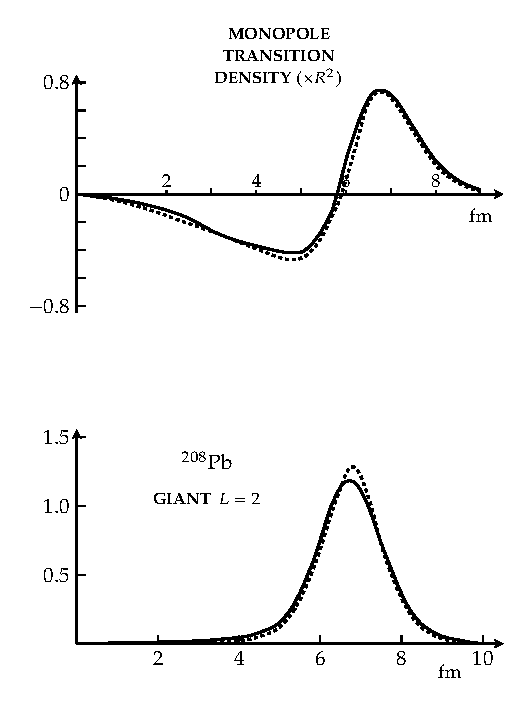
\includegraphics[width=0.8\textwidth]{pictures/8_14}
\par\end{centering}
\caption{\label{fig:8_14}$^{208}\mathrm{Pb}$ 中的同位旋标量单极与四极跃迁密度（引自 \cite{BT75}）。虚线为简单流体动力学公式，实线为连续谱
RPA 计算结果。}
\end{figure}

\ref{fig:8_14} 表明流体动力学公式（虚线）与自洽连续谱 RPA 计算（实线）展现出惊人的吻合，这无可辩驳地证实了巨共振在本质上对应着经典核液滴的表面振动与体压缩振动。

一个典型的例子是 $^{208}\mathrm{Pb}$ 中的低激发集体 $3^{-}$ 态。\ref{fig:8_15} 展示了其实验与理论的径向跃迁密度
$\rho^{0}(r)$。实验测量值与 Bohr-Tassie 模型的宏观预测存在相当剧烈的偏离。而通过求解包含密度依赖有效力的微观
RPA 方程所得到的理论曲线，与实验数据达成了极其优良的吻合。对于高激发的 $3^{-}$ 巨八极共振，其与 Bohr-Tassie
模型的吻合则再次恢复良好［St 79］。

\begin{figure}[H]
\begin{centering}
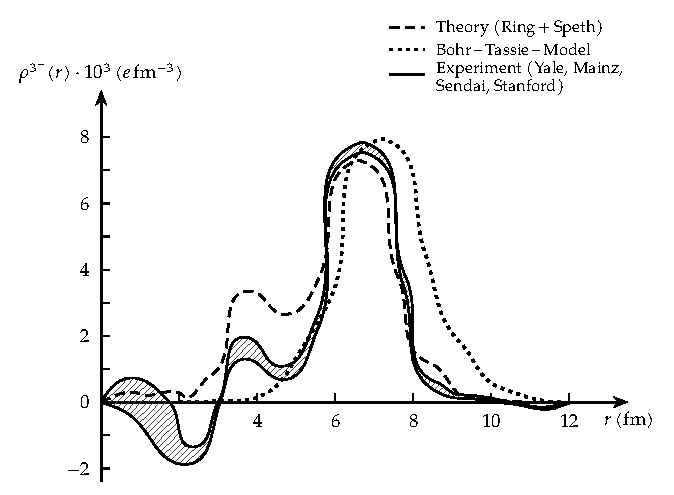
\includegraphics[width=0.7\textwidth]{pictures/8_15}
\par\end{centering}
\caption{\label{fig:8_15}$^{208}\mathrm{Pb}$ 最低 $3^{-}$ 态的理论与实验径向跃迁密度。实线标示了实验误差范围［RFM
74］，虚线［TW 73］基于采用 Migdal 力的 RPA 计算，点线对应于 Bohr-Tassie 模型（引自 \cite{St79}）。}
\end{figure}


\section{粒子-粒子 RPA\label{sec:8.8_=007C92=005B50-=007C92=005B50_RPA}}

\subsection{形式理论\label{subsec:8.8.1_=005F62=005F0F=007406=008BBA}}

正如在 Tamm-Dancoff 方法中我们区分粒子-空穴与粒子-粒子 TDA（第 8.2.3 节）一样，对应于 ph RPA，我们同样拥有粒子-粒子（pp）RPA。对于
$A+2$ 系统的本征态 $|\tau\rangle$，类比于 ph 拟设 (\ref{eq:rpa_creation_operator})，我们有：

\begin{equation}
|A+2,\tau\rangle=R^{\dagger}_{\tau}|A,0\rangle\label{eq:pprpa_state_ansatz}
\end{equation}

属于 $A$ 体系的基态由下式定义：

\begin{equation}
R_{\tau}|A,0\rangle=0\label{eq:pprpa_vacuum_def}
\end{equation}

在与式 (\ref{eq:rpa_xy_amplitudes_density}) 相同的准玻色子近似下，我们得到：

\begin{align}
X^{\tau}_{mn} & =\langle A,0|a_{n}a_{m}|A+2,\tau\rangle,\nonumber \\
Y^{\tau}_{ij} & =\langle A,0|a_{j}a_{i}|A+2,\tau\rangle\label{eq:pprpa_amplitudes_def}
\end{align}

利用 $R^{\dagger}_{\tau}$ 的运动方程，完全类比于 ph 情形（第 8.4.1 节），我们导出 $A+2$
核系统相对于 $A$ 核基态的激发能 $\hbar\Omega_{\tau}=E^{A+2}_{\tau}-E^{A}_{0}$
所满足的方程［FIS 64, Sch 64b, MLE 67, Ro 68a, b, RP 69］：

\begin{equation}
(\hbar\Omega_{\tau}-\epsilon_{m}-\epsilon_{n})X^{\tau}_{mn}=\sum_{m'<n'}\bar{v}_{mnm'n'}X^{\tau}_{m'n'}+\sum_{i'<j'}\bar{v}_{mni'j'}Y^{\tau}_{i'j'}\label{eq:pprpa_plus2_eq}
\end{equation}

对于 $A-2$ 粒子系统，我们同样得到完全对应的方程：

\begin{equation}
(\hbar\Omega_{\lambda}+\epsilon_{i}+\epsilon_{j})Y^{\lambda}_{ij}=-\sum_{i'<j'}\bar{v}_{iji'j'}Y^{\lambda}_{i'j'}-\sum_{m'<n'}\bar{v}_{ijm'n'}X^{\lambda}_{m'n'}\label{eq:pprpa_minus2_eq}
\end{equation}

式中 $\hbar\Omega_{\lambda}=E^{A}_{0}-E^{A-2}_{\lambda}$。由此，我们可以将方程
(\ref{eq:pprpa_plus2_eq}) 与 (\ref{eq:pprpa_minus2_eq}) 合并为一个类似于
ph 形式的紧凑矩阵方程：

\begin{equation}
\begin{pmatrix}A & B\\
B^{\dagger} & C
\end{pmatrix}\begin{pmatrix}X^{\tau}\\
Y^{\tau}
\end{pmatrix}=\hbar\Omega_{\tau}\begin{pmatrix}1 & 0\\
0 & -1
\end{pmatrix}\begin{pmatrix}X^{\tau}\\
Y^{\tau}
\end{pmatrix}\label{eq:pprpa_matrix_eq}
\end{equation}

式中（$m<n,\,m'<n',\,i<j,\,i'<j'$）：

\begin{align}
A_{mnm'n'} & =(\epsilon_{m}+\epsilon_{n})\delta_{mm'}\delta_{nn'}+\bar{v}_{mnm'n'},\nonumber \\
C_{iji'j'} & =-(\epsilon_{i}+\epsilon_{j})\delta_{ii'}\delta_{jj'}-\bar{v}_{iji'j'},\nonumber \\
B_{mnij} & =\bar{v}_{mnij}\label{eq:pprpa_matrix_blocks}
\end{align}

需要指出的是，Hermitian 矩阵 $A$ 与 $C$ 通常具有不同的维度，矩阵 $B$ 因而是一个长方阵。方程 (\ref{eq:pprpa_matrix_eq})
同时给出了 $A+2$ 与 $A-2$ 系统的本征态，这与 ph 情形不同（在 ph 情形中所有解属于相同粒子数的系统）。然而，这并不意味着
pp RPA 破坏了粒子数守恒（如 BCS 模型所做的那样），拟设 (\ref{eq:pprpa_state_ansatz}) 严格保持粒子数。在实践中，我们可以根据波函数的振幅特征识别出属于
$A+2$ 体系的解：它们具有很大的 pp 分量 $X_{mn}$ 与极小的 hh 分量 $Y_{ij}$，能量位于 $\epsilon_{m}+\epsilon_{n}$
能区。

pp-RPA 本征矢满足如下归一化与完备性关系：

\begin{equation}
\sum_{m<n}X^{\tau*}_{mn}X^{\tau'}_{mn}-\sum_{i<j}Y^{\tau*}_{ij}Y^{\tau'}_{ij}=\delta_{\tau\tau'}\label{eq:pprpa_orthonormality}
\end{equation}

\begin{equation}
\sum_{\tau}\left(X^{\tau}_{mn}X^{\tau*}_{m'n'}-Y^{\tau}_{mn}Y^{\tau*}_{m'n'}\right)=\delta_{mm'}\delta_{nn'}\label{eq:pprpa_closure}
\end{equation}


\subsection{对振动诱发的基态关联\label{subsec:8.8.2_=005BF9=00632F=0052A8=008BF1=0053D1=007684=0057FA=006001=005173=008054}}

利用 Thouless 定理，pp RPA 基态同样可表示为指数形式：

\begin{equation}
|\text{RPA}\rangle=N_{0}\exp\left(\sum_{m<n,\,i<j}Z_{mnij}A^{\dagger}_{mn}A_{ij}\right)|\text{HF}\rangle\label{eq:pprpa_ground_state_correlated}
\end{equation}

式中 $A^{\dagger}_{mn}=a^{\dagger}_{m}a^{\dagger}_{n}$，$A_{ij}=a_{j}a_{i}$，且
$Z=Y^{*}X^{*-1}$。展开式 (\ref{eq:pprpa_ground_state_correlated}) 可以看出，关联基态除
$|\text{HF}\rangle$ 外还包含了带有成对玻色子的虚激发，由于 pp 玻色子数目严格等于 hh 玻色子数目，粒子数是严格守恒的。

对于纯配对力 $-G$，式 (\ref{eq:pprpa_matrix_eq}) 导出如下色散关系：

\begin{equation}
\frac{2}{G}=\sum_{n}\frac{2j_{n}+1}{2\epsilon_{n}-\hbar\Omega}+\sum_{i}\frac{2j_{i}+1}{2|\epsilon_{i}|+\hbar\Omega}\label{eq:pprpa_pairing_dispersion}
\end{equation}

当配对力常数 $G$ 增大至临界值：

\begin{equation}
G_{\text{crit}}=\frac{2}{\sum_{n}\frac{2j_{n}+1}{2\epsilon_{n}}+\sum_{i}\frac{2j_{i}+1}{2|\epsilon_{i}|}}\label{eq:pprpa_gcrit_def}
\end{equation}

时，最低集体对振动的激发能 $\hbar\Omega\to0$，标志着正常核系统发生向超流态（BCS 凝聚）的相变。在 $G>G_{\text{crit}}$
时，BCS 能隙方程具有非零解 $\Delta>0$，此时必须采用准粒子表象。

\section{准粒子 RPA（QRPA）\label{sec:8.9_=0051C6=007C92=005B50RPA=00FF08QRPA=00FF09}}

在远离闭壳层时，配对关联极其重要，使得配对场对单粒子运动的反馈不再能够忽略。我们在第 6 章和第 7 章已经看到，在这些情形下，采用
BCS 或 HFB 基态是恰当的。由于它也是一个广义行列式波函数，我们可以完全类比于正常系统构造 TDA 和 RPA 理论［Ba 60a］。由此将显现出：粒子-空穴
RPA 与粒子-粒子 RPA 可以被统一包容于一个紧凑的准粒子 RPA（QRPA）方程之中［So 71］。

为了推导这些方程，我们从准粒子表象下的 Hamiltonian 量［式 (E.18)］出发：

\begin{equation}
H=H^{0}+H^{11}+H^{20}+H^{40}+H^{31}+H^{22}\label{eq:qrpa_h_quasiparticle_decomp}
\end{equation}

准粒子声子算符定义为：

\begin{equation}
Q^{\dagger}_{\nu}=\sum_{k<k'}\left(X^{\nu}_{kk'}\alpha^{\dagger}_{k}\alpha^{\dagger}_{k'}-Y^{\nu}_{kk'}\alpha_{k'}\alpha_{k}\right)\label{eq:qrpa_phonon_creation_def}
\end{equation}

类比于第 8.4.1 节的推导，我们得到准粒子 RPA 方程，其矩阵形式与式 (\ref{eq:rpa_matrix_equation})
完全一致：

\begin{equation}
\begin{pmatrix}A & B\\
B^{*} & A^{*}
\end{pmatrix}\begin{pmatrix}X^{\nu}\\
Y^{\nu}
\end{pmatrix}=\hbar\Omega_{\nu}\begin{pmatrix}1 & 0\\
0 & -1
\end{pmatrix}\begin{pmatrix}X^{\nu}\\
Y^{\nu}
\end{pmatrix}\label{eq:qrpa_matrix_equation}
\end{equation}

唯独此时矩阵指标遍历组态空间中的所有准粒子对 $(k<k')$。矩阵 $A$ 和 $B$ 给定为（$k<k',\,l<l'$）：

\begin{align}
A_{kk'll'} & =\langle\text{HFB}|[\alpha_{k'}\alpha_{k},[H,\alpha^{\dagger}_{l}\alpha^{\dagger}_{l'}]]|\text{HFB}\rangle=(E_{k}+E_{k'})\delta_{kl}\delta_{k'l'}+H^{22}_{kk'll'},\nonumber \\
B_{kk'll'} & =-\langle\text{HFB}|[\alpha_{k'}\alpha_{k},[H,\alpha_{l'}\alpha_{l}]]|\text{HFB}\rangle=H^{40}_{kk'll'}\label{eq:qrpa_ab_matrices_def}
\end{align}

它们共同构成了 HFB 理论的稳定性矩阵［式 (7.37)］。在时间反演不变的规范基下，矩阵元可以利用 Bogoliubov 变换的
$u,v$ 系数显式计算：

\begin{align}
A_{kk'll'} & =(E_{k}+E_{k'})\delta_{kl}\delta_{k'l'}+\bar{v}_{kl'k'l}(u_{k}v_{k'}u_{l}v_{l'}+v_{k}u_{k'}v_{l}u_{l'})+\cdots,\nonumber \\
B_{kk'll'} & =\bar{v}_{kk'll'}(u_{k}u_{k'}v_{l}v_{l'}+v_{k}v_{k'}u_{l}u_{l'})+\cdots\label{eq:qrpa_uv_coefficients_explicit}
\end{align}

在 Hartree-Fock 极限下（所有 $u=0,1$），QRPA 方程自动退化并解耦为通常的粒子-空穴 RPA 方程与粒子-粒子
RPA 方程。

准粒子 RPA 方程已广泛应用于结合可分离相互作用（如配对加四极模型、表面 $\delta$ 相互作用）的研究中。它不仅能够成功描述球形超导核中的低激发集体振动，而且能够成功应用于形变稀土核和锕系核中
$\beta$ 振动、$\gamma$ 振动、八极振动以及配对振动的微观描述；同时通过结合推转自洽模型，亦能很好地描述伴随其上的转动带结构与形变核中的巨共振现象。
